
\chapter{Introducción al magnetismo} % Main chapter title

%----------------------------------------------------------------------------------------

% Define some commands to keep the formatting separated from the content 
\newcommand{\keyword}[1]{\textbf{#1}}
\newcommand{\tabhead}[1]{\textbf{#1}}
\newcommand{\code}[1]{\texttt{#1}}
\newcommand{\file}[1]{\texttt{\bfseries#1}}
\newcommand{\option}[1]{\texttt{\itshape#1}}
\newcommand{\grados}{$^{\circ}$}

%----------------------------------------------------------------------------------------



\vspace{0.5cm} 

\begin{flushright}
Yo prefiero ese algo recóndito que alguien del sexo opuesto emitía hacia mi.\\
A ese algo voy a llamarlo aquí “magnetismo”.\\
Una fuerza que te atrae y absorbe, te guste o no te guste, quieras o no\\
Al sur de la frontera, al oeste del Sol\\
Haruki Murakami
\end{flushright}
\vspace{1.0cm} 


 

%$\centerdot$ Creo que lo mas didáctico es desarrolla la primera parte del curso a través de las similitudes que poseen los materiales \textbf{piezomagnéticos} y \textbf{piezoeléctricos}. Si bien los fenómenos no son exactamente iguales poseen algunas similitudes, luego tratamos de explicar el fenómeno magnético Para tal fin exponemos un brevísimo resumen de la mecánica cuántica, ya que el magnetismo atómico es un fenómeno cuántico.
%
%$\centerdot$ En un material piezomagnético, uno puede inducir un momento magnético espontáneo al
%aplicar una tensión mecánica, o bien una deformación física aplicando un campo magnético El \textbf{piezomagnetismo} es un fenómeno que se caracteriza por un acoplamiento lineal entre la polarización magnética y la tensión mecánica.
%
%$\centerdot$  Los materiales piezoeléctricos son aquellos que al ser sometidos a tensiones mecánicas,
%adquiere una polarización eléctrica, luego generan una diferencia de potencial en su superficie.
%
%$\centerdot$ Actualmente se piensa que el piezomagnetismo es un efecto magnetomecánico lineal análogo al efecto electromecánico lineal de la piezoelectricidad De igual manera, la magnetostricción y la electroestricción son efectos análogos de segundo orden. Estos efectos de orden superior se pueden pensarse de primer orden si las variaciones de los parámetros son pequeñas"
%
%Algo realmente importante en estos fenómenos es que son reversibles como se representa en la figura \ref{fig:10}
%
%
%\begin{figure}[H]
%    \centering
%    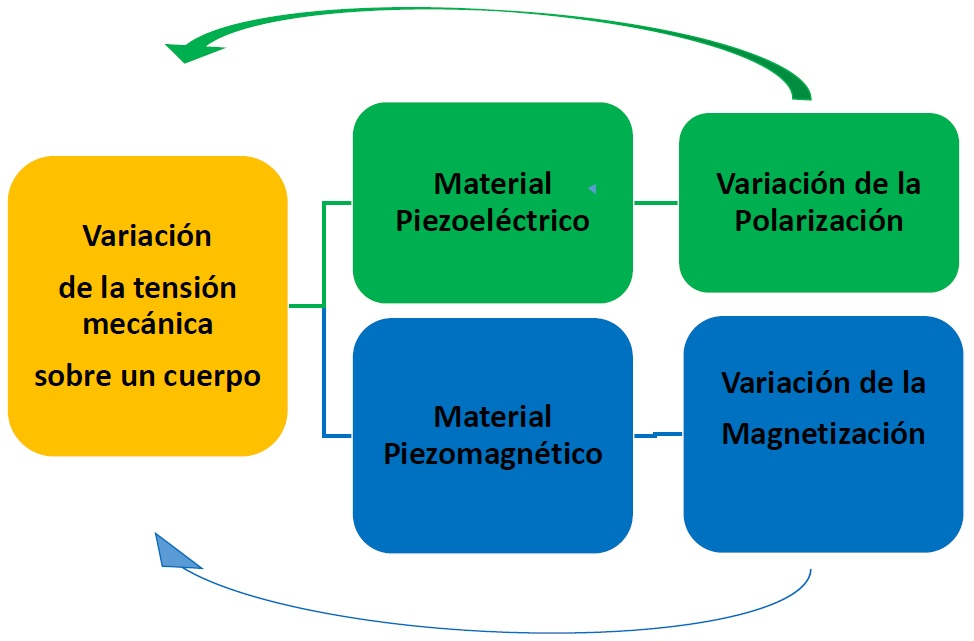
\includegraphics[width=0.80\textwidth]{./Figures/fig10}
%	\caption{Efectos piezoeléctrico y piezomagnético}
%	\label{fig:10}
% \end{figure}
%
%
%\begin{figure}[H]
%    \centering
%    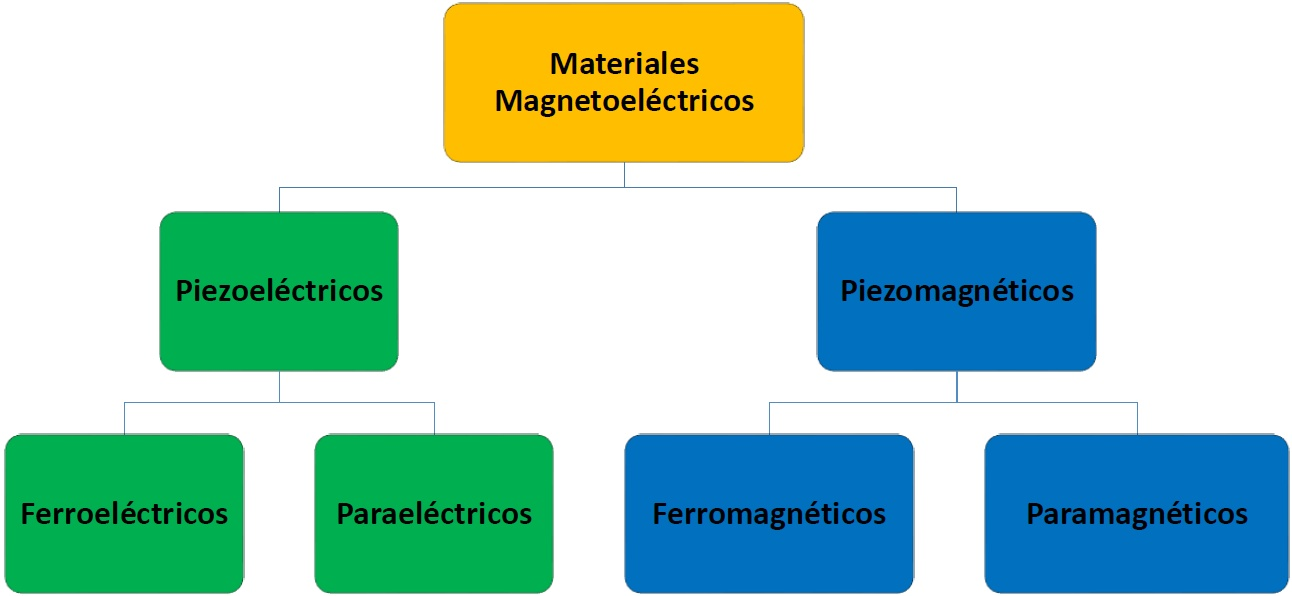
\includegraphics[width=1.0\textwidth]{./Figures/fig11}
%	\caption{Materiales magnetoeléctricos}
%	\label{fig:10}
% \end{figure}
%
%Tratemos de explicar el origen de estos dos fenómenos recordando algunas ideas

\section{Introducción histórica} 

$\centerdot$ Iniciamos este trabajo con un breve e incompleto resumen histórico sobre la idea de átomo.

\begin{itemize}
\item \textbf{Joseph John Thomson} recibió el Premio Nobel de Física en 1906 por el descubrimiento del \textbf{electrón en 1897} Thomson probó que los rayos catódicos tenían naturaleza corpuscular y estaban formados por electrones Curiosamente, su hijo \textbf{George Pagget Thomson} también recibió el Premio Nobel de Física en 1937 por demostrar que el electrón es una onda constituyendo la demostración experimental de la dualidad partícula onda

\item Se atribuye a \textbf{Ernest Rutherford} el descubrimiento del \textbf{protón, en el año 1918} con carga positiva e igual a la del electrón ($1,6\times 10^{-19}$C) Es una partícula subatómica cuya masa e 1836 veces superior a la del electro En la década del 1970 se crean evidencia que es una partícula compuesta.

\item \textbf{James Chadwick} descubre el \textbf{neutrón en el año 1932}, partícula que no tiene carga eléctrica y que junto con el protón constituye el núcleo atómico Su masa es similar a la del protón Fuera del núcleo el neutrón es inestable dura $14,7$ minutos El neutrón es el responsable de la estabilidad de los núcleos.

\item A lo largo de la historia la idea de átomo fue cambiando, desde la propuesta de Dalton en adelante, cada nuevo modelo explicaba algún fenómeno, fallando en otros, ya que nacen de experiencias realizadas. Solo comentaremos los mas recientes.

\item \textbf{J. J. Thomson} luego del descubrimiento del electrón propuso en 1898 que los átomos son esferas de materia con carga positiva embebida de electrones.

\item \textbf{E. Rutherford en 1911} describe al átomo como compuesto por un núcleo, pequeño, de carga positiva con los electrones a cierta distancia exterior
girando, con gran cantidad de espacio vacío La importancia de este modelo es que introducía la existencia de un nucleo atómico.

\item \textbf{Modelo de Niels Bohr en 1913} supone que solo algunas órbitas de los electrones son posibles, con esta hipótesis logra explicar los espectros de emisión y absorción atómicos. Este modelo es clásico pero introduce por primera ves ideas de cuántica. Supuso que los electrones solamente se podían mover en órbitas circulares definidas. Cada órbita puede ser identificada mediante un número entero \textbf{n} llamado número cuántico principal.

\item \textbf{Arnold Sommerfeld en 1916} presenta el modelo atómico de Bohr modificado donde introduce orbitas de los electrones elípticas y velocidades relativistas. La excentricidad de la orbita dio lugar al número cuántico azimutal, que establece la forma de los orbitales, se lo representa con la letra \textbf{l} y toma valores que van desde $0$ hasta $n-1$.

\item \textbf{Modelo de Schrödinger 1926} plantea una ecuación de onda para los electrones, que los supone ondas de \textbf{De Broglie}. La solución estacionaria de ecuación de Schrödinger del átomo esta caracterizada por tres números cuánticos \textbf{n}, \textbf{l} y \textbf{m}. Predice adecuadamente las líneas espectrales de distintos tipos de átomos, tanto neutros como ionizados y explica las uniones químicas. Posteriormente \textbf{Max Born 1926} propone la interpretación probabilística de la función de onda de los electrones y \textbf{Dirac en 1928} generaliza la ecuación de Schrödinger agregando la relatividad y dando origen al espín del electrón y su numero cuántico \textbf{s}. Hasta aquí es todo lo que necesitamos saber para entender el átomo.

\end{itemize}


%\section{Tipo de interacción elemental y similitudes}
%\textbf{Dipolo eléctrico}, reacciona ante un $\V{E}$ externo orientándose en la dirección de éste. A grandes distancias del dipolo la intensidad del campo $\V{E}$ disminuye $\left( \dfrac{1}{r^{3}}\right)$ con mayor rapidez que el campo eléctrico eléctrico $\left( \dfrac{1}{r^{2}}\right)$ de una sola partícula cargada.
%
%\begin{figure}[H]
%    \centering
%    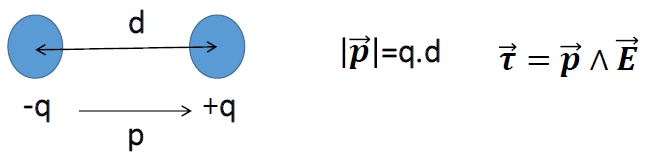
\includegraphics[width=0.80\textwidth]{./Figures/fig12}
%	\caption{Dipolo Eléctrico}
%	\label{fig:13}
% \end{figure}
%
%\textbf{Dipolo magnético} reacciona ante un campo $\V{H}$ externo orientándose en dirección a éste
%También aquí a grandes distancias del dipolo la intensidad del campo $\V{B}$ disminuye $\left( \dfrac{1}{r^{3}}\right)$
%
%\begin{figure}[H]
%    \centering
%    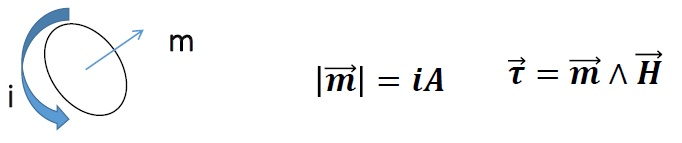
\includegraphics[width=0.80\textwidth]{./Figures/fig13}
%	\caption{Dipolo Magnético}
%	\label{fig:13}
% \end{figure}
%
%\subsection{Dipolos eléctricos y magnéticos}
%
%\begin{itemize}
%
%\item Se ve que existe una coincidencia entre el campo eléctrico creado por dos cargas eléctricas de signo contrario y el campo magnético engendrado por una corriente circular en un anillo, siempre que los miremos desde lejos Luego no fue necesario pensar en la existencia de monopolos magnéticos El dipolo magnético se genera por el movimiento de una carga eléctrica.
%
%\item En el caso de cargas eléctricas la existencia del momento dipolar es un testimonio de la asimetría de la estructura de cargas.
%
%\item Existen átomos o moléculas aisladas que poseen un momento dipolar magnético espontaneo, similarmente hay átomos o moléculas aisladas que poseen un momento dipolar eléctrico estos son llamados paramagnéticos o paraeléctricos respectivamente.
%
%\item El descubrimiento del efecto piezoeléctrico en el cuarzo, dará la posibilidad de generar y recepcionar sonidos a voluntad Este hallazgo fue realizado por los hermanos Pierre y Jacques Curie en 1881 Un tiempo antes 1842 James Prescott Joule descubre el fenómeno piezomagnéticos Este fenómeno tiene características similares al piezoeléctrico Se tardó unos años en encontrar aplicaciones concretas a estos dos fenómenos.
%
%\end{itemize}
%
%\subsection{Formación de los dipolos eléctricos}
%
%\textbf{Dieléctrico}: Es un material mal conductor de electricidad, por lo que puede ser utilizado como aislante eléctrico, además si es sometido a un campo eléctrico externo, puede establecerse en él un campo eléctrico interno No hay cargas libres Todos los materiales dieléctricos son aislantes pero no todos los materiales aislantes son dieléctricos En general hay dos tipos de materiales dieléctricos los que las moléculas, iones o átomos son polares y las que se polarizan por la existencia del campo eléctrico Existen varios mecanismos por intermedio de los cuales se polarizan los materiales, no entraremos en mas detalles.
%
%\begin{figure}[H]
%  \centering
%  \begin{minipage}[b]{0.47\textwidth}
%    \centering
%     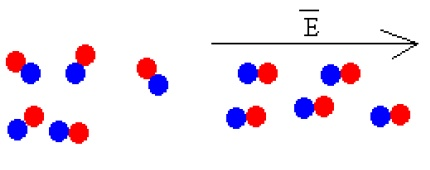
\includegraphics[width=1.0\textwidth]{./Figures/fig14}
%	 \caption{\protect\raggedright Moléculas polares.}
%	\label{fig:14}
%  \end{minipage}
%  \hfill
%  \begin{minipage}[b]{0.47\textwidth}
%    \centering
%     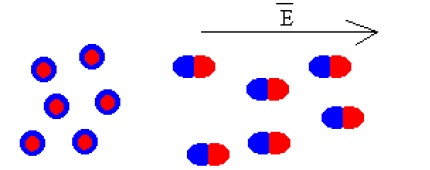
\includegraphics[width=1.0\textwidth]{./Figures/fig15}
%	 \caption{\protect\raggedright Moléculas no polares.}
%	\label{fig:15}
%  \end{minipage}
%\end{figure}
%
%
%La molécula de agua, tiene una distribución asimétrica de sus electrones, lo que la convierte en una molécula polar, alrededor del oxígeno se concentra la nube de carga negativa, mientras que los núcleos de hidrógeno quedan desprovistos parcialmente de sus electrones, luego, manifiestan, una densidad de carga positiva Por tanto la molécula de agua es dipolar Las moléculas polares pueden formar compuestos químicos, cuando interactúan entre si, las fuerza que manifiestan los dipolos se llama de fuerza de Van der Waals.

\section{Formulación matemática}

Maxwell logra, en el siglo 19 expresar matemáticamente los hallazgos de Faraday y engloba todos los fenómenos clásicos del electromagnetismo en sus ecuaciones, concibe las ondas electromagnéticas y determina su velocidad


\begin{equation*}
\label{eq:100}
\begin{aligned}
	\nabla \times \overrightarrow{H} = \overrightarrow{J_{c}} + \dPv{D}{t} 
	\quad \quad
	&\nabla \times \overrightarrow{E} = - \dPv{B}{t} 	\\
	\nabla \cdot \overrightarrow{B}=0
	\quad \quad
	&\nabla \cdot \overrightarrow{D} = \rho_{l}
\end{aligned}
\end{equation*}

\begin{equation*}
	\V{f}= q(\V{E}+\V{v}\times\V{B})
\end{equation*}

Se ve que una corriente eléctrica genera un campo magnético, dicho de otro modo el movimiento de cargas eléctricas genera un campo magnético, luego existe una relación entre movimiento de cargas y campo magnético, ¿que podría explicar el magnetismo atómico?

$\V{E}$ Campo eléctrico en el espacio, $\V{D}$ Denota efectos eléctricos en la materia \\
$\V{H}$ Campo magnético en el espacio, $\V{B}$ Campo magnético en la materia \\
$\V{f}$ fuerza de Lorentz.

Parecería que con las ecuaciones de Maxwell se tendría la descripción total del magnetismo atómico. !No es así¡ El magnetismo en los sólidos es un fenómeno cuántico. Muchos de los fenómenos magnéticos solo se pueden explicar cuánticamente Un modelo atómico Borh simple considera al electrón girando alrededor del núcleo atómico muy pequeño El núcleo contiene toda la carga positiva del átomo Las ecuaciones de Maxwell sugieren que un electro acelerado debe radiar energía con una frecuencia fundamental y otras armónicas múltiplo de la fundamental Si el movimiento del electrón es circular (y por tanto acelerado) y uniforme, emitiría una sola frecuencia, luego el electrón perdería energía y colapsaría Tampoco podemos explicar la estabilidad del núcleo atómico con tantas cargas positivas juntas

Sabemos que los fenómenos de óptica se deben tratar de dos maneras distintas según el caso si la dimensión del objeto es mucho mayor que la longitud de onda de la luz, podemos utilizar la óptica geométrica y definir trayectorias bien precisas, la luz se la trata como una partícula, por el contrario si la longitud de onda de la luz es comparable con la dimensión del objeto, aparecen los fenómenos de difracción y no se puede utilizar la óptica geométrica No podemos definir una trayectoria ni afirmar que son partículas Si aceptamos este tipo de comportamiento para el micro mundo, entonces la longitud $\lambda$ de un determinado ente esta dada por la expresión:

\begin{equation}
	\lambda=\dfrac{h}{mv}
\end{equation}

Donde $h\approx 6,62607015 \times 10^{-34}\left[ Js\right]$ es la constante de Planck, $m$ la masa y $v$ la velocidad.

Veamos si tiene sentido tratar a una bolita de $1gr$ que se mueve a una velocidad de $1\frac{cm}{s}$ como una onda, calculando $\lambda=6,6\times10^{-27}cm$. Totalmente despreciable frente al tamaño del cuerpo. Tendremos fenómenos de difracción en zonas de dimensiones comparables con las longitudes de onda. Si realizamos el mismo calculo para los átomos vemos que la longitud de onda es comparable a la dimensión atómica, por tanto, debemos abandonar la idea de trayectoria del electrón bien definida girando a una distancia fija del núcleo. Veamos otro ejemplo:

Supongamos electrones en un tubo de RX que son acelerados con una diferencia de potencial de $10kV$ luego:

\begin{equation}
	eV = h \nu = h\dfrac{c}{\lambda}
\end{equation}


De donde $\lambda$ será:

\begin{equation}
	\lambda =\dfrac{ch}{eV} = 1.239\times 10^{-10} m
\end{equation}

Esto lleva a pensar que la materia tiene propiedades de partícula y de onda, lo que comúnmente se llama dualidad partícula onda pero ¡no significa que sean al mismo tiempo las dos cosas!. Estas ondas se llaman ondas de De Broglie o de materia. Lo único que podemos afirmar es que todo ente en
movimiento, bajo cierto experimento se comporta como onda y bajo otro experiencia como particular Tengamos en cuenta que estos fenómenos nos son percibidos directamente por nuestros sentidos En la figura \ref{fig:16} tenemos las tres proyecciones de un objeto que esta dentro de la esfera, ¿quien puede decir que es?. 

\begin{figure}[H]
    \centering
    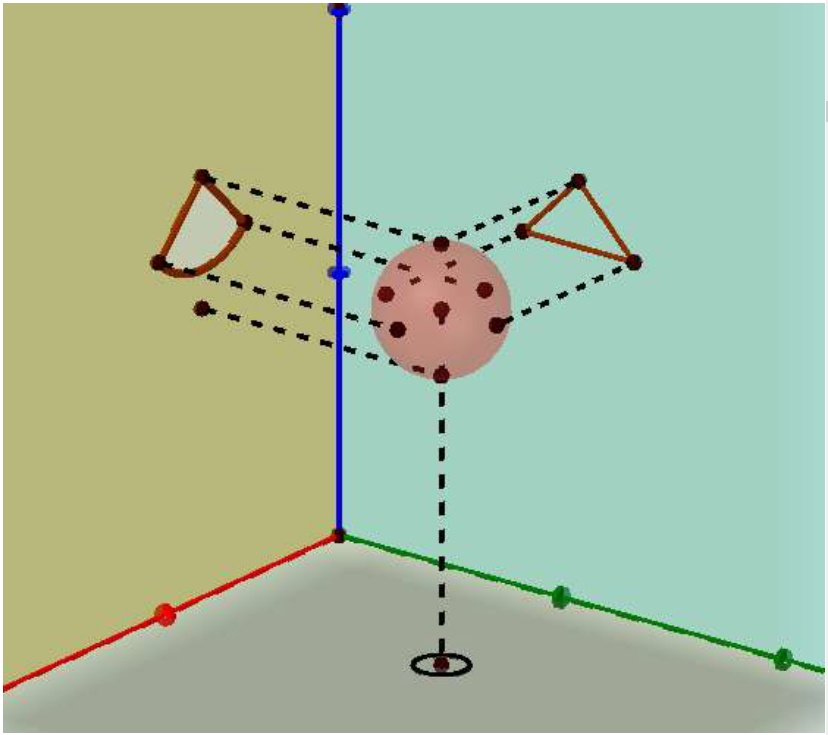
\includegraphics[width=0.80\textwidth]{./Figures/fig16}
	\caption{Proyecciones en tres planos}
	\label{fig:16}
 \end{figure}


Las características ondulatoria y corpuscular son complementarias y excluyentes, nuestro conocimiento de las particularidades es parcial si solo utilizamos uno de ellos. 

No debemos explicar el micromundo en función de conceptos del macromundo como son las ondas puras o partículas puras, solo será posible comprender el átomo si pensamos en el comportamiento corpuscular de las ondas y en el comportamiento ondulatorio de las partículas.

¿Como hallamos esta onda de De Broglie que caracteriza el fenómeno?, por intermedio de la ecuación
diferencial de Schrödinger La solución de esta ecuación nos da lo que llamamos función de onda $\Psi$  que en un punto del espacio y en un instante de tiempo nos da la probabilidad de encontrar la entidad en ese lugar e instante.

La solución de la ecuación de Schrödinger es normalmente un problema complicado Sin embargo, su solución dio excelentes resultados y predijo fenómenos observados experimentalmente imposibles de explicar con la física clásica. Mencionemos un par de ejemplos:

1.- La ecuación Schrödinger independiente del tiempo, para un caso unidimensional tiene el
siguiente aspecto:

\begin{equation}
	\dfrac{d^{2}\Psi}{dx^{2}} + \dfrac{2m}{\hbar^{2}}\big( E-V(x) \big)\Psi = 0
\end{equation}

Donde $m$ es la masa, $V(x)$ la energía potencial, $E$ la energía total del sistema y $\hbar=\dfrac{h}{2\pi}$. La solución de la ecuación no solo depende de la función $V(x)$ sino también del valor numérico de $E$. Para cualquier valor de $E$ no es posible encontrar una solución $\Psi$ continua y con condiciones de probabilidad, luego se comprueba que solo hay solución para valores discretos de la energía $E_{1}$, $E_{2}$, $E_{3}, \cdots E_{n}$. La energía toma valores discretos, esta
cuantificada y se los llama valores propios, siendo $\Psi_{1}$, $\Psi_{2}$, $\Psi_{3}, \cdots \Psi_{n}$ las funciones propias o características

2.- Suponiendo ahora un pozo cuadrado de potencial como el que se muestra en la figura \ref{fig:17}
Resolviendo la ecuación de Schrödinger para este potencial, se observa los niveles de energía en color
azul y en rojo una función propia particular, indicando que existe la posibilidad de encontrar al ente
fuera del pozo, fenómeno observado en los núcleos radiactivos que emiten partículas alfa Efecto que
no se explica en la mecánica clásica, efectivamente, ya que

\begin{equation}
	E=\dfrac{m}{2}v^{2} + V \therefore v= \sqrt{\dfrac{2}{m}\left( E-V(x) \right)} 
\end{equation}

\begin{figure}[H]
    \centering
    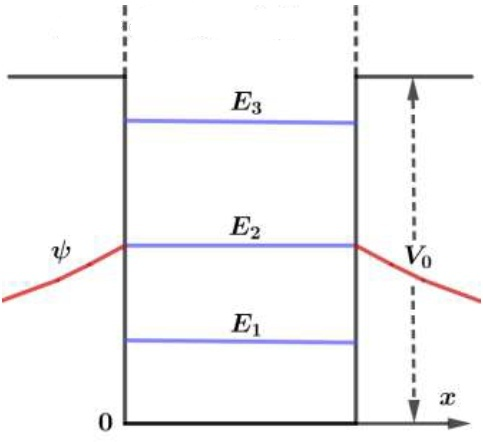
\includegraphics[width=0.60\textwidth]{./Figures/fig17}
	\caption{Pozo de potencial}
	\label{fig:17}
 \end{figure}

Dentro
del pozo $E>V$ ya que el potencial es cero, pero fuera tiene el valor $V_{0}>E$ por tanto la velocidad $v$ seria imaginaria, lo que no tiene sentido, luego clásicamente no podría salir del pozo.

Si el potencial es infinito (paredes totalmente rígidas), caso que no se da en la practica, no se debe
esperar penetración fuera del pozo

3.- Efecto túnel, este fenómeno es también netamente cuántico no apreciado en la mecánica clásica, por ejemplo, si tenemos electrones confinados por una barrera de potencial, únicamente aquellos electrones que excedan en energía la barrera de potencial podrán escapar, clásicamente Si por medio de la ecuación de Schrödinger calculamos la probabilidad de encontrar un electrón del otro lado de la barrera veremos que esta probabilidad no es cero.

\begin{equation}
	\dfrac{\vert\Psi_{b}\vert^{2}}{\vert\Psi_{a}\vert^{2}} \approx e^{-2\sqrt{\dfrac{2m(V_{0}-E)}{\hbar^{2}}}\,W} 
\end{equation}

\begin{figure}[H]
    \centering
    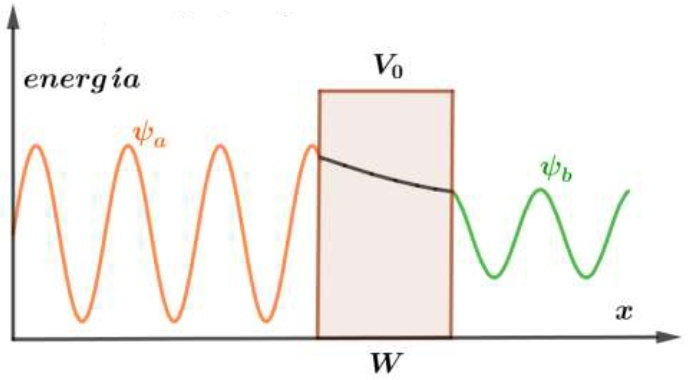
\includegraphics[width=0.80\textwidth]{./Figures/fig18}
	\caption{Efecto túnel}
	\label{fig:18}
 \end{figure}

\section{Números cuánticos}

Estamos en condiciones de entrar en la teoría cuántica atómica y entender el origen del magnetismo atómico, como también, comprender la tabla periódica de los elementos y las uniones químicas. Para ello pensemos en un campo central de fuerza, eléctricas, el mas simple, un protón como núcleo y un electrón, átomo de hidrogeno, como en el modelo de Bohr. En un campo central electrostático sabemos que el potencial depende solo de la distancia al centro. Resolviendo la ecuación de Schrödinger en el espacio (es fácil decirlo) se encuentran tres números cuánticos, alguno de ellos coincide con lo postulado por Bohr Por tanto, los podemos enumerar.

\begin{itemize}
	\item[1]$n=1, 2, 3, \cdots$ número cuántico principal
	\item[2]$l=0, 1, 2, \cdots (n-1)$ número cuántico orbital
	\item[3]$m_{l}=0, \pm 1,\pm 2, \cdots \pm l$ número cuántico magnético
\end{itemize}

\textbf{Número cuántico principal $n$}
La energía del átomo de hidrogeno se cuantifica con el número $n$ por una expresión similar a la supuesta por Bohr

\begin{equation}
	E_{n}= \dfrac{me^{4}}{8\epsilon_{0}^{2}h^{2}} \left(\dfrac{1}{n^{2}} \right) 
\end{equation}

Como vemos no es posible tomar cualquier energía.

\textbf{Número cuántico orbital $l$}

Sabemos que en la mecánica Newtoniana el momento angular en un campo central se mantiene constante con el tiempo a medida que el sistema va cambiando y está dado por la expresión:

\begin{equation}
	\V{L}= \V{r} \times \V{p} = \V{r} \times m \V{v} 
\end{equation}

Luego puede variar la velocidad y $\V{r}$ de cualquier forma, si se manteniendo constante $\V{L}$ En mecánica cuántica al igual que la energía también se conserva el momento angular Las leyes clásicas de conservación tienen su equivalente cuántico, hay leyes de conservación cuántica que no tienen
análogo clásico El número cuántico $l$ informa de la cuantificación del módulo del momento angular del electrón en su órbita dado por la expresión:

\begin{equation}
	\vert\V{L}\vert = \sqrt{l(l+1)} \hbar
\end{equation}

Vemos que la unidad natural del momento angular es $\hbar= 1,054 \times 10^{−34}[Js]$.

Generalmente y como un legado de la espectroscopia se designa a los valores de $l$ con letras en minúscula de tal manera que $l=0\rightarrow s$, $l=1\rightarrow p$, $l=2\rightarrow d$. Un estado $s$ tiene momento angular cero, un estado $p$ tiene momento angular $2\hbar$ El vector $\V{L}$ es perpendicular al plano que contiene el movimiento.

\textbf{Número cuántico magnético $m_{l}$}

La componente del momento angular en una dirección determinada, por ejemplo $z$ es $L_{z}$ y esta determinada por el numero cuántico magnético $m_{l}$ por medio de la expresión siguiente: 

\begin{equation}
	L_{z}= m_{l} \hbar
\end{equation}

Luego la componente $L_{z}$ del momento angular no se orienta en cualquier dirección del espacio, esta cuantificada, como $m_{l}$ puede ser positivo o negativo hay ($2l+1$) orientaciones del vector $\V{L}$. En mecánica clásica, como fue dicho, el $\V{L}$ en un campo central es constante en modulo y dirección, en cuántica solo conocemos el modulo y una componente $L_{z}$ lo que impide conocer la dirección exacta de $L$ Como solo podemos conocer $\vert\V{L}\vert$ y $L_{z}$ imaginamos al vector $\V{L}$ realizando una precesión alrededor del eje $z$.
 
Supongamos el caso de $l=2$ entonces será:

\begin{equation*}
	\vert\V{L}\vert = \sqrt{l(l+1)} \hbar = \sqrt{6}\hbar = 2,45\hbar
\end{equation*}



%Comenzaremos estudiando el magnetismo en átomos, iones, moléculas, para luego pasar a los sólidos. El magnetismo es un fenómeno netamente cuántico en el sentido que debe ser explicado desde esta teoría, sin embargo, unos pocos fenómenos pueden explicase con la física clásica y así lo haremos.
%
%Nuestro mundo macroscópico está constituido por cuerpos y ondas, los cuerpos a su vez por partículas. Tenemos una clara noción de lo que llamamos partícula y onda, las vemos la sentimos y las tocamos. En el caso del mundo microscópico nada de esto es factible, solo es posible interpretar algo a través del comportamiento. ¿Qué otra imagen del micro mundo podemos construir si solo conocemos partículas y ondas?, pero ¿realmente que es? o sea la esencia no lo conocemos. Se trata de interaccionar con el sistema estudiado y de acuerdo a su respuesta interpretar como está constituido.
%
%La Mecánica Cuántica logra describir correctamente los fenómenos atómicos, es decir, en correspondencia con el experimento. De esta manera nace y se desarrolla la mecánica cuántica.
%
%Sin tener nada que ver con nuestro tema y aludiendo a cuestiones filosóficas, mucho tiempo antes de que se gestara la mecánica cuántica (1612), Galileo Galilei escribe una carta a un amigo diciendo: “\textit{Non tentare le essenze, ma contentarsi delle affezioni quantitative}”\footnote{No investigar la esencia, sino contentarse con los efectos cuantitativos}, lo cual es aplicable, también, a nuestro caso.
%%----------------------------------------------------------------------------------------
%
%%\section{Contexto y motivación.}
%
%\section{Magnetismo de iones y átomos libres}
%
%\begin{itemize}
%	\item El magnetismo es un fenómeno cuántico, muchos de los fenómenos magnéticos solo se pueden explicar cuánticamente.
%	\item Un modelo atómico simple considera al electrón girando alrededor del núcleo atómico, esto genera un momento angular orbital $\overrightarrow{\textit{L}}$, podemos tener una imagen bastante real si consideramos al electrón
%girando sobre si mismo, esto genera el momento angular de espín $\overrightarrow{\textit{S}}$. Son dos momentos angulares distintos.
%	\item Es conocido que una corriente eléctrica genera un campo magnético, dicho de otro modo el movimiento de cargas eléctricas genera un campo magnético, luego existe una relación entre movimiento de cargas y campo magnético.
%
%	\item Esta relación es generada por que el electrón posee carga eléctrica y un momento magnético. Este fenómeno posibilitara aplicaciones que se verán más adelante (materiales ferroicos).
%	\item Es en esta relación donde debemos buscar el origen atómico del magnetismo.
%\end{itemize}
%
%
%\subsection{Momento angular orbital}
%
%El momento angular orbital $\overrightarrow{\textit{L}}$ es un vector con módulo:
%
%\begin{equation}
% |\overrightarrow{L}| = \sqrt{l \big(l+1\big) } \, \frac{h}{2 \pi } = \sqrt{l \big(l+1\big) } \, \hbar 
%\end{equation}

Las distintas posiciones del vector $\V{L}$ en el espacio están definidas por el número cuántico orbital $l$ que toma valores entre:

\begin{equation}
 l = 0, 1, 2, 3 \ldots\big(n-1\big) \quad y \quad \hbar = \frac{h}{2 \pi }
\end{equation}


La proyección del vector $\overrightarrow{\textit{L}}$ respecto del eje $z$ en el espacio están definidas por el número cuántico magnético $m_{l}$ que varía entre:

\begin{equation}
 -l,\ldots,0 ,\ldots, +l \quad \text{o sea:} \quad -2,-1,0,+1,+2
\end{equation}

El valor del vector $\V{L_{z}}$ (la dirección del eje $z$ es determinada por un campo magnético externo), está dada por la expresión:

\begin{equation}
	L_{z}=m_{l}\hbar
\end{equation}

Donde $m_{l}$ varia $m_{l}=0, \pm 1, \pm 2, \pm 3, \cdots, \pm l$

\begin{figure}[H]
    \centering
    \includegraphics[width=0.60\textwidth]{./Figures/Gráfico3}
	\caption{Momento angular sus proyecciones}
	\label{fig:Grafico3}
\end{figure}

Para conocer exactamente la dirección de $\V{L}$ es necesario conocer no solo $L_{z}$, si no también $L_{x}$ y $L_{y}$, pero, la Mecánica Cuántica demuestra que es imposible conocer mas de una componente de $\V{L}$. Observemos que $\V{L}$ nunca puede tener la dirección de $z$ o sea coincidir con el campo
magnético, en ese caso conoceríamos las tres componentes.

En la figura \ref{fig:129} tenemos una representación más realista que la anterior.

\begin{figure}[H]
    \centering
    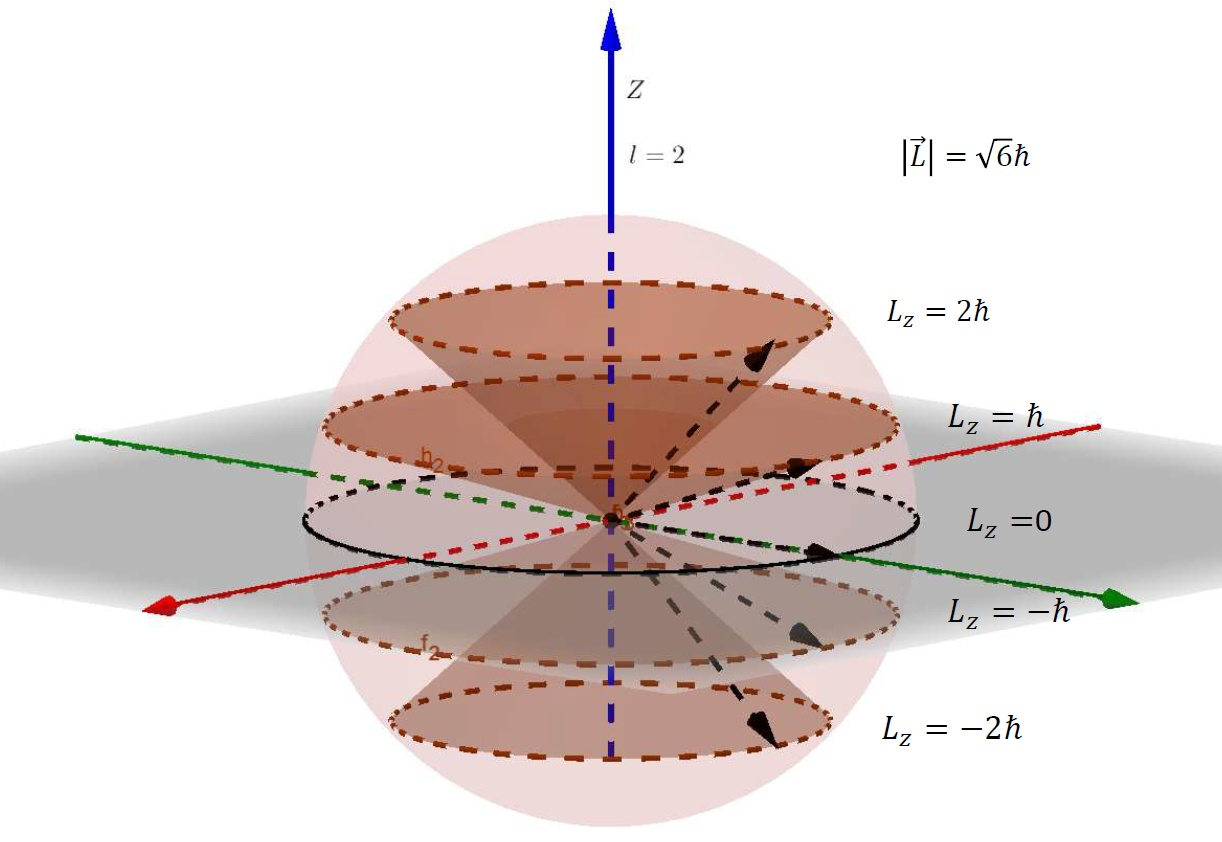
\includegraphics[width=1.0\textwidth]{./Figures/fig129}
	\caption{Momento angular sus proyecciones en 3D}
	\label{fig:129}
\end{figure}

\textbf{Número cuántico $s$}

Un tema aparte es el llamado espín. Este es esencialmente cuántico y hace referencia a una característica intrínseca (i.e. inherente; se refiere a una propiedad física de las partículas subatómicas, por la cual toda partícula elemental o compuesta que se comporte como elemental tiene un momento angular intrínseco de valor fijo Se trata de una propiedad individual de la partícula como lo es la masa o la carga eléctrica). El espín no sale naturalmente de la solución de la ecuación de Schrödinger, que vimos anteriormente. Por supuesto que fue necesario introducirlo para lograr una descripción completa de determinadas observaciones espectrales y entender a los átomos con mas de un electrón En el año 1928 P. Dirac propuso una ecuación cuántica relativista, desde la cual se deriva naturalmente la existencia del espín. P. Dirac pensaba que toda ley física debería tener belleza matemática o sea simetría, generalidad, Esta particularidad tenía su ecuación, lo cual implicaba una novedosa consecuencia, la existencia de una partícula simétrica al electrón con igual masa y similar carga eléctrica, pero positiva. Esta partícula cuando se encuentra con su simétrica un electrón se aniquila liberando la energía de ambas partículas en forma de rayos $\gamma$. Dirac, sin conocerla ni haberla visto profetizo la existencia de la antimateria, tan solo fue sugerida por su ecuación matemática y la idea de simetría. Carl Anderson descubre la primera antipartícula en 1932.

Al espín los podemos interpretar como el momento angular intrínseco de la partícula en reposo. Llamamos $\V{S}$ al espín del electrón y su modulo será

\begin{equation}
 |\V{S}| = \sqrt{s \big(s+1\big) } \, \frac{h}{2 \pi } = \sqrt{s \big(s+1\big) } \,\hbar 
\end{equation}

Expresión similar a la del momento orbital $|\V{L}|$, donde $s$ es el número cuántico de espín, cuyo valor es $\frac{1}{2}$ para el electrón. También se lo mide en unidades de $\hbar$.
 
\begin{equation}
 |\V{S}| = \sqrt{s \big(s+1\big) } \, \frac{h}{2 \pi } = \frac{\sqrt{3}}{2}\, \hbar
\end{equation}

Esto no tiene nada de clásico, el modulo adquiere un solo valor y si lo interpretamos como el momento angular obserbamos que no puede modificar su velocidad de giro, clásicamente inexistente.

También aquí la componente $S_{z}$ del momento angular de espín de un electrón a lo largo del eje $z$ determinada por un campo magnético exterior está cuantificada y puede tomar dos valores según el número cuántico magnético de espín $m_{s}$, para $m_{s}=+\dfrac{1}{2}$ y $m_{s}=-\dfrac{1}{2}$:

\begin{equation}
 S_{z} = m_{s} \hbar = \pm \frac{1}{2} \hbar
\end{equation}

En la figura \ref{fig:Gráfico2corregido} se observa las posiciones posibles del vector momento angular del electrón:

\begin{figure}[H]
    \centering
    \includegraphics[width=0.60\textwidth]{./Figures/Gráfico2corregido}
	\caption{Momento angular de espín y sus proyecciones}
	\label{fig:Gráfico2corregido}
\end{figure}

Estas propiedades no pueden ser explicadas por modelos clásicos. Si se explican combinando ideas de la Mecánica Cuántica y la Relatividad. (Dirac , 1928)\footnote{En 1928 Dirac reformula el tratamiento de Schrödinger para el átomo monoelectrónico de tal forma que las ecuaciones fueran consistentes con los requerimientos de la teoría de la relatividad. De las soluciones a las ecuaciones de Dirac surgían, de forma natural, los tres números cuánticos ya conocidos $(n, l, ml)$ más un cuarto número cuántico $(s)$ relacionado con esta propiedad intrínseca del electrón que denominamos espín.}.











En mecánica clásica el $\V{L}$ en un campo central es constante en modulo y dirección, en cuántica solo conocemos el modulo y una componente $L_{z}$, lo que impide conocer la dirección exacta.
Como solo podemos conocer $|\V{L}|$ y $L_{z}$ imaginamos al vector $\V{L}$ realizando una precesión alrededor del eje $z$




\subsection{Momento magnético orbital del electrón}

Los momentos angulares de partículas cargadas tiene asociado un momento magnético, cuyo sentido es opuesto al del vector $\V{L}$. Según el electromagnetismo el momento magnético asociado al momento angular orbital del electrón es (como se verá)

\begin{equation}
	\V{\mu_{l}} = \frac{-e\hbar}{2m} \, \V{L}= -\mu_{B} \V{L}
\end{equation}

donde $e$ es la carga del electrón y $m$ la masa del electrón en reposo y $\mu_{B}=\dfrac{e\hbar}{2m}$ es llamado Magnetón de Bohr (unidades atómicas del momento magnético). El signo $–$ significa que los vectores tienen sentido contrarios. Pasando a modulo:

\begin{equation}
 |\overrightarrow{\mu_{l}}| = \sqrt{l \big(l+1\big) } \,  \frac{-e\hbar}{2m} = \sqrt{l \big(l+1\big) } \, \mu_{B} 
\end{equation}

La proyección del momento magnético orbital en la dirección de $z$ es:

\begin{equation}
	\mu_{l_{z}} = -m_{l}\mu_{B}
\end{equation}

\begin{figure}[H]
    \centering
    \includegraphics[width=0.60\textwidth]{./Figures/Gráfico1}
	\caption{Momento angular y momento magnético orbital}
	\label{fig:Grafico1}
 \end{figure}

El electrón en su orbita puede pensarse como un imán solo si $l\neq 0$, si $l=0$ no existe trayectoria, tiene $\vert\V{L}\vert$ en su estado fundamental.


\subsection{Momento magnético del spín del electrón}

Para el electrón, que tiene carga y momento angular se podría espera algo similar a lo obtenido con el momento magnético orbital Sin embargo la expresión clásica no se cumple cuánticamente y es necesario multiplicar por un factor llamado $g_{e}$  de Landé, cuyo valor según Dirac es $g_{e}=2$. Luego el momento magnético del espín es \textbf{exactamente el doble que la del electrón en su movimiento orbital}.

\begin{equation}
	\V{\mu_{S}} = g_{e} \dfrac{-e\hbar}{2m}\V{S} = -g_{e}\mu_{B}\V{S}
\end{equation}

Pasando a modulo:

\begin{equation}
	\vert\V{\mu_{S}}\vert = \sqrt{s(s+1)} \dfrac{e\hbar}{m} = \dfrac{e\sqrt{3}}{2m} \hbar = \sqrt{3} \mu_{B}
\end{equation}

La proyección de este momentos magnético de espín, según una dada dirección del espacio z determinada por un campo magnético externo es:

\begin{equation}
	{\mu_{S}}_{z} = -m_{S} \mu_{B}
\end{equation}

En este caso $m_{S}=\pm \dfrac{1}{2}$, o sea que toma solo dos valores. Estamos en presencia de un imán elemental, \textbf{en la mayoría de los casos el electrón puede ser considerado como un imán elemental}.

Si bien introducimos algunas ideas de la física cuántica no se realizo una demostración exacta de los resultados presentados. En la mayoría de los casos los esquemas son semi cuánticos y las expresiones matemáticas también. Es el momento de presentar el momento magnético del electrón en su movimiento orbital y el del electrón asociado al espín. Si aceptamos una hipótesis del electromagnetismo clásico que indica que los momentos angulares de partículas cargadas tienen asociado un momento magnético, cuyo sentido es opuesto al del vector momento angular. Ver figura \ref{fig:113}

\begin{figure}[H]
    \centering
    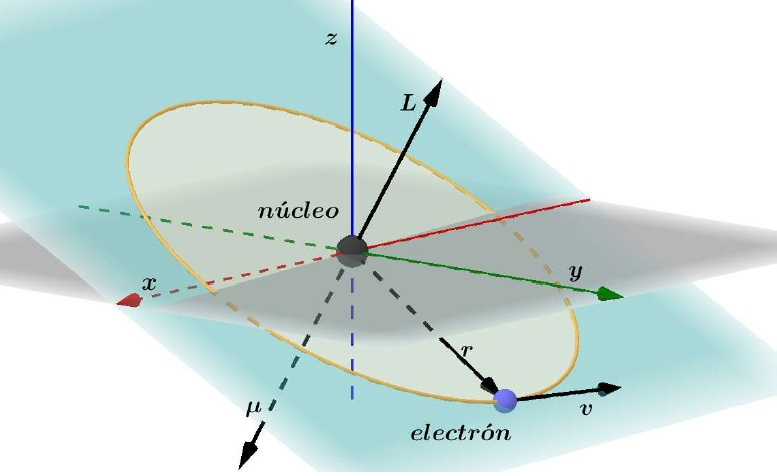
\includegraphics[width=0.9\textwidth]{./Figures/fig113}
	\caption{Momento angular del electrón}
	\label{fig:113}
 \end{figure}

En el caso del momento magnético orbital es aceptable la imagen clásica del electrón con carga eléctrica que al girar genera el momento magnético Para el caso del momento magnético del espín en el electrón, también podríamos aceptar que su momento angular genera un momento magnético, pero la hipótesis clásica se pierde al ver que el momento magnético de espín existe en partículas sin carga, como el fotón y el neutrón. Sin embargo estas suposiciones son de suma utilidad para explicar efectos macroscópicos del magnetismo, y otros fenómenos como la resonancia magnética nuclear En la figura \ref{fig:114} se muestra un esquema del espín y del momento angular orbital en un átomo La magnitud de los vectores no son reales

\begin{figure}[H]
    \centering
    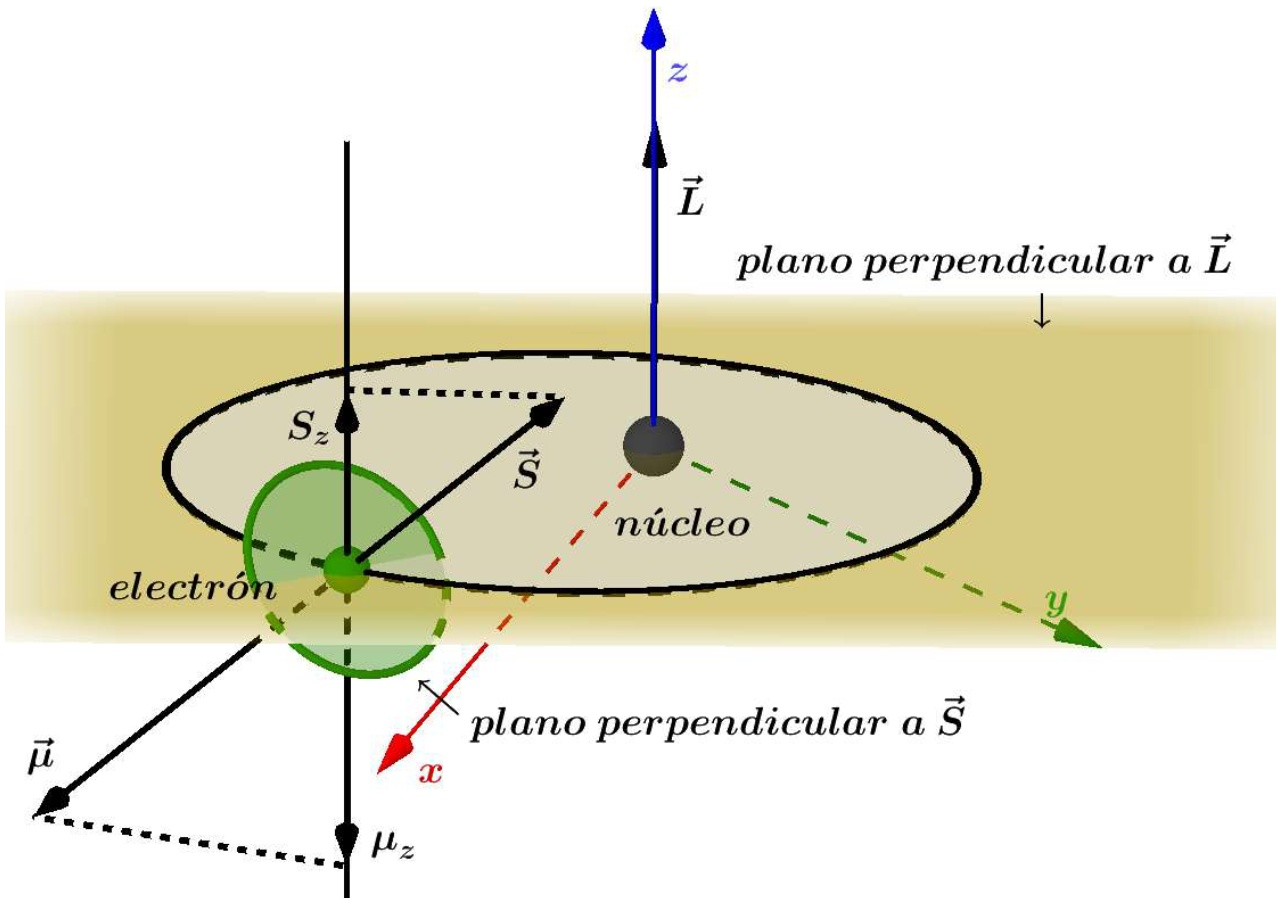
\includegraphics[width=0.9\textwidth]{./Figures/fig114}
	\caption{Espín y momento angular}
	\label{fig:114}
 \end{figure}


Para el electrón, que es una partícula cargada, se podría espera algo similar a lo obtenido en el momento magnético orbital, pero no, el momento magnético de espín, al igual que la masa o la carga del electrón, es una propiedad intrínseca fundamental\footnote{Existen partículas neutras sin carga eléctrica como el neutrón que sin embargo tienen momento magnético (de hecho el neutrón no se considera realmente elemental sino formado por tres quarks cargados fraccionariamente)}. Si fuera el caso clásico su valor seria 1 pero en realidad es un poco mayor de 2 (da exactamente 2 aplicando la ecuación de Dirac y con la corrección de los efectos cuánticos del campo electromagnético un poco más de 2).


\begin{figure}[H]
    \centering
    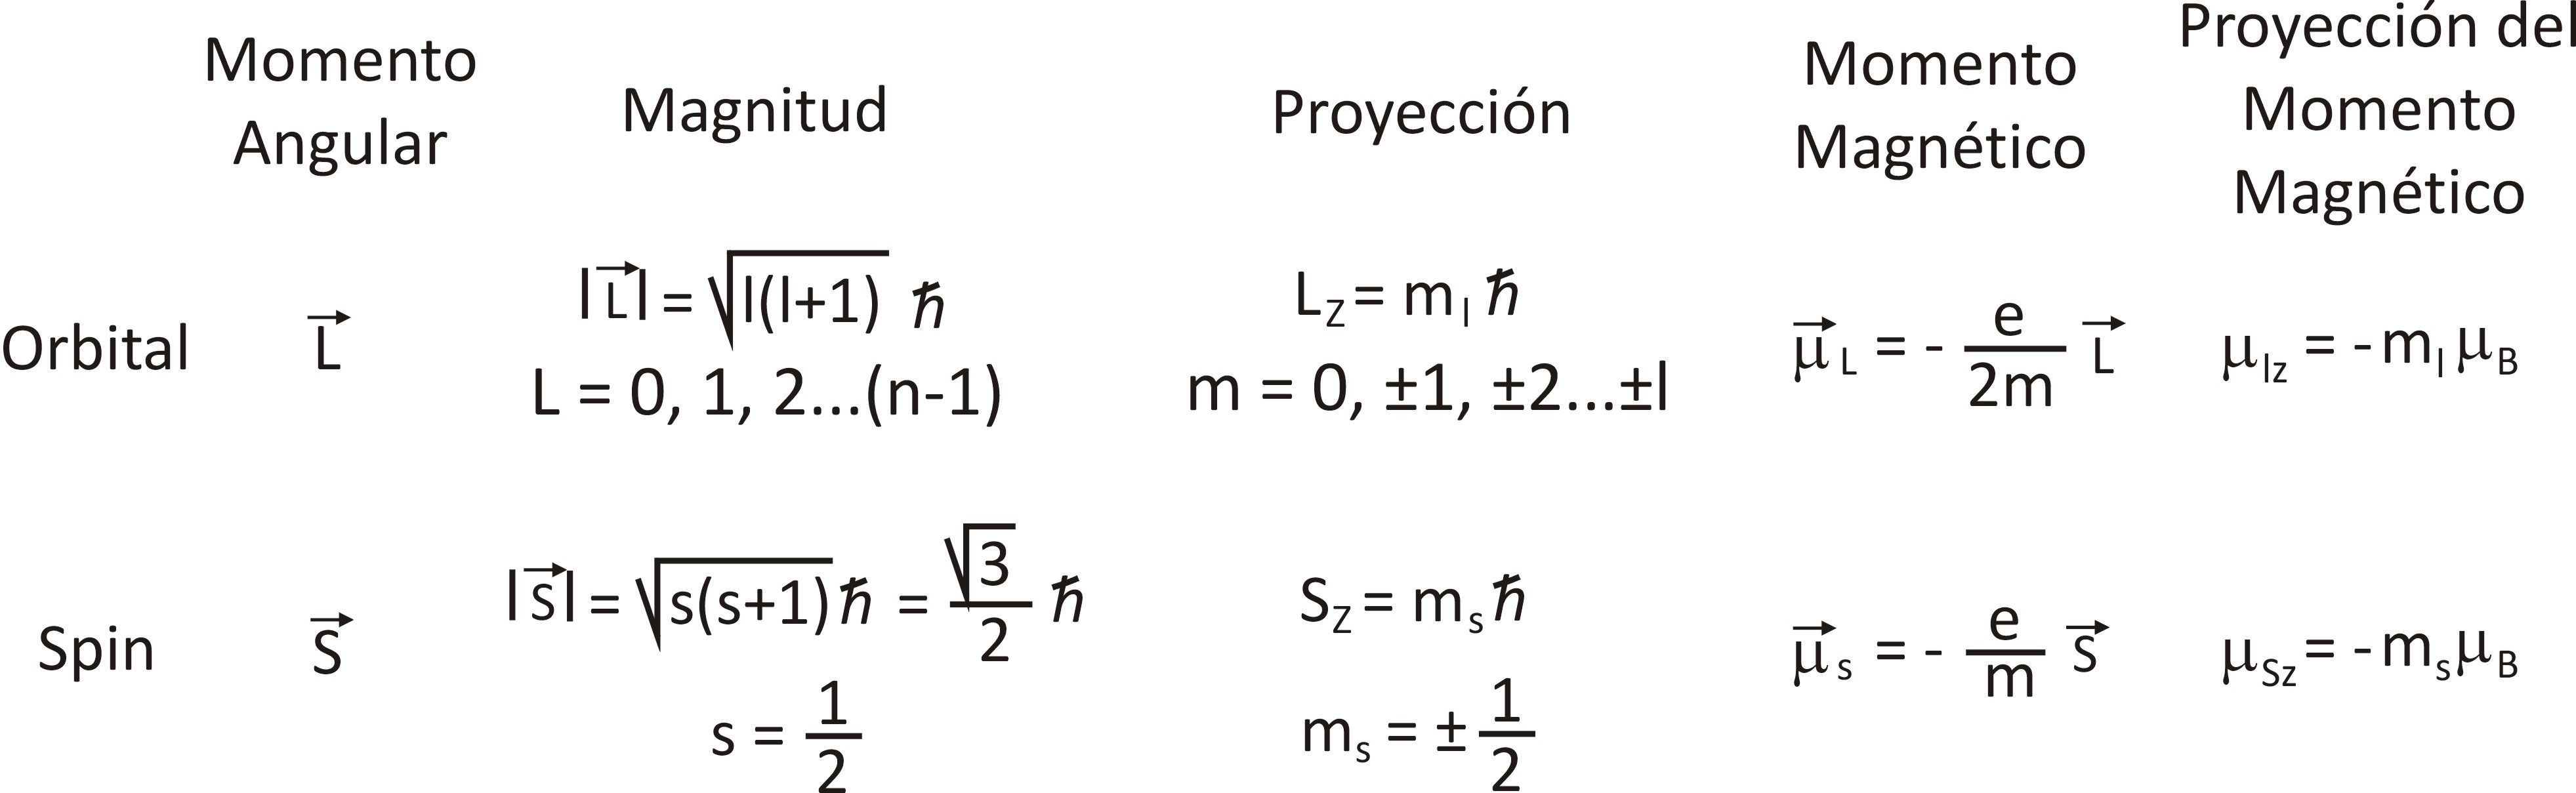
\includegraphics[width=1.0\textwidth]{./Figures/LyS}
	\caption{Resumen de números cuánticos}
	\label{fig:GraficoLyS}
\end{figure}

\textbf{Ejemplo:}

Calculemos los ángulos que forman $L_{z}$ y el vector $\overrightarrow{L}$, en nuestro caso $l = 2$


\begin{equation}
  sin \big(\alpha\big)=\frac{L_{z}}{|\V{L}|}=\frac{m_{l}\,\hbar}{\sqrt{l(l+1)} \, \hbar}=\begin{cases}
  				m_{l}=2 \rightarrow\alpha\approx 46^{\circ} \\
  				m_{l}=1 \rightarrow\alpha\approx 24^{\circ} \\  				
  				m_{l}=0 \rightarrow\alpha=0^{\circ} \\
  				m_{1}=-1 \rightarrow\alpha\approx 336^{\circ} (-24^{\circ})\\
  				m_{1}=-2 \rightarrow\alpha\approx 314^{\circ} (-46^{\circ})
    			\end{cases}
\end{equation}

El vector momento angular orbital nunca puede estar alineado al campo magnético, ya que ello requeriría que el ángulo $\alpha$ tomase un valor de $90^{\circ}$ o de $270^{\circ} (-90^{\circ})$, para lo cual se requeriría que:

\begin{equation}
 \frac{m_{l}}{\sqrt{6}}= \pm1 \quad \text{y por lo tanto} \quad m_{l}=\pm\sqrt{6}= \pm2,45
\end{equation}

Mayor que el valor $m_{l}\leq|2|$ en este caso. Por otro lado, si es coincidente con la dirección del campo conoceríamos las tres componentes de vector momento angular orbital, lo cual está prohibido.

Seguimos trabajando con el átomo de hidrogeno es decir con un solo electrón. Recordemos que el tratamiento que hacemos es semi cuántico. Cuando es posible, y si el resultado clásico no difiere mucho del cuántico utilizamos el modelo clásico.

\section{Interacción espín órbita L-S}

Vimos que un electrón en un átomo tiene un momento angular orbital $\V{L}$ y también un momento angular $\V{S}$ estos momentos pueden interactuar y acoplarse, se la llama interacción espín órbita (L-S) Luego, sumando vectorialmente los dos momentos se encuentra el momento angular total del átomo llamado $\V{J}$. No consideramos el momento angular del núcleo por ser varios miles de veces menor que la interacción L-S Luego, lo definimos como $\V{J}=\V{L}+\V{S}$. Este debe cumplir con las mismas propiedades que los momentos angulares $\V{L}$ y $\V{S}$.Es decir, debe ser ejecutado de acuerdo a los lineamientos de la mecánica cuántica La interacción L-S, es muy débil en el átomo de hidrógeno, pero muy importante en átomos con más electrones 

$\vert \V{J} \vert = \sqrt{J(J+1)}\hbar$, donde $J$ es el numero cuántico correspondiente.

En general $J$ varia desde $(l-s), (l-s+1), \cdots, (l+s-1), (l+s)$ luego para un electrón $\vert l-\dfrac{1}{2}\vert \leq j \leq \vert l+\dfrac{1}{2}\vert$ luego $j=l \pm \dfrac{1}{2}$. Mientras que $J_{z}=m_{j}\hbar$.
 
Analicemos como se puede realizar la suma e indaguemos si puede ser arbitrara el ángulo que forman los vectores. Para eso consideremos el siguiente esquema y aplicamos el teorema del coseno.

\begin{equation}
	J^{2}=L^{2}+S^{2}-2\,L\,S\,Cos(\alpha)
\end{equation}

Los módulos de los vectores se miden en unidades de $\hbar$, luego reemplazando los módulos:

\begin{equation}
	j(j+1)=l(l+1)+s(s+1)-2\,\sqrt{l(l+1)}\,\sqrt{s(s+1)}\,Cos(\alpha)
\end{equation}

Por lo tanto:

\begin{equation}
	Cos(\alpha) = \dfrac{j(j+1)-l(l+1)-s(s+1)}{2\,\sqrt{l(l+1)}\,\sqrt{s(s+1)}}
\end{equation}

Donde vemos que el valor del ángulo no puede ser cualquiera y depende de los números cuánticos $l$ y $s$ ya que el numero cuántico $j$ también depende de los anteriores. Se ve que para un valor fijo de $l$,  $j$ puede tomar solo dos valores $j=l \pm \dfrac{1}{2}$, luego hay solo dos valores del ángulo para cada $l$. Estos dos estados tiene una pequeña diferencia de energía y es lo que genera la llamada estructura fina de las líneas espectrales.

Veamos un ejemplo: 

Primero para $l=1$, $s=+\dfrac{1}{2}$. Calculamos los módulos de los vectores para $j=1+s=\dfrac{3}{2}$ luego construimos la suma conociendo los lados

\begin{equation*}
	\begin{aligned}[c]
		&\qa{j}=\dfrac{3}{2}\big(\dfrac{3}{2}+1\big)= \dfrac{15}{4}\\
		&\qa{l}=2\\
		&\qa{s}=\dfrac{3}{4}
	\end{aligned}
\qquad\Longrightarrow\qquad
	\begin{aligned}[c]
		&\lv{J} = \qa{j} = \sqrt{\dfrac{15}{4}} = 1,90\\
		&\lv{L} = \qa{l} = \sqrt{2} = 1,41\\
		&\lv{S} = \qa{s} = \sqrt{\dfrac{3}{4}} = 0,86
	\end{aligned}
\end{equation*}

Por el teorema del coseno podemos verificar que el ángulo es el correcto. Recordemos que todo se mide en unidades de $\hbar$

Ahora calculemos $l=1$, $s=-\dfrac{1}{2}$, los valores absolutos de $l$ y $s$ no cambian y ahora  hacemos el calculo con el teorema del coseno:

\begin{equation}
	\begin{aligned}[c]
	Cos(\alpha) =& \dfrac{j(j+1)-l(l+1)-s(s+1)}{2\,\sqrt{l(l+1)}\,\sqrt{s(s+1)}} = \dfrac{\qa{\dfrac{1}{2}}-2-\dfrac{3}{4}}{2\sqrt{2}\sqrt{\dfrac{3}{4}}}=\\
	&\dfrac{-2}{2,44}=-0,81\Rightarrow \alpha = 143^{o}
	\end{aligned}
\end{equation}


mientras que el modulo de $\lv{J}$ es igual a $\qa{l}=\qa{\dfrac{1}{2}}=\sqrt{\dfrac{3}{4}}=0,86$ tal como se ve representado en la figura \ref{fig:115}. Vemos que si el átomo tiene un solo electrón hay solo dos orientaciones posibles: en la primera $\lv{J}>\lv{L}$ mientras que en la segunda $\lv{J}<\lv{L}$.


\begin{figure}[H]
    \centering
    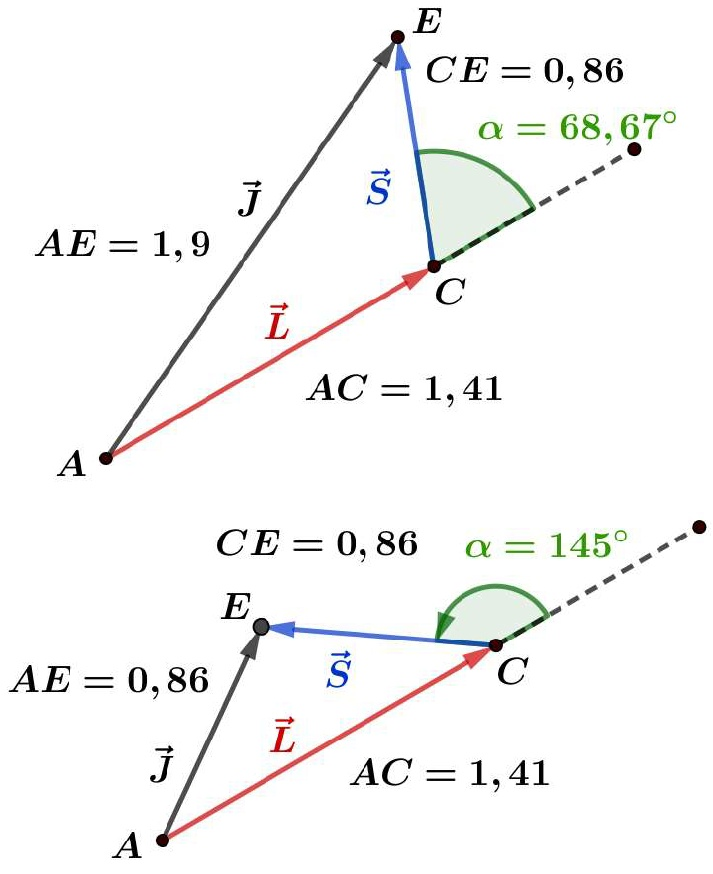
\includegraphics[width=0.6\textwidth]{./Figures/fig115}
	\caption{Interacción L-S}
	\label{fig:115}
 \end{figure}

En ausencia de campo magnético externo, el momento angular total del átomo $\V{J}$ se conserva, es decir modulo y dirección constante, en tanto $\V{L}$ y $\V{S}$ rotaran al rededor de $\V{J}$. Por supuesto, para el átomo de hidrógeno con un solo electrón.

Si ahora aplicamos un campo $\V{B}$ exterior débil, de manera que no rompa la interacción espín orbita (L-S). Será $\V{J}$ quien rote alrededor del campo eterno sin romper la iteración (L-S), luego seguirán rotando $\V{L}$ y $\V{S}$ alrededor de $\V{J}$. La orientación de $\V{J}$ en el campo externo $\V{B}$  deberá cumplir con uno de los valores permitidos de $m_{j}$. Si se aumenta el campo magnético externo se rompe el acoplamiento (L-S) y dejan $\V{L}$ y $\V{S}$ de rotar alrededor de $\V{J}$. Observe la figura \ref{fig:116} 


\begin{figure}[H]
    \centering
    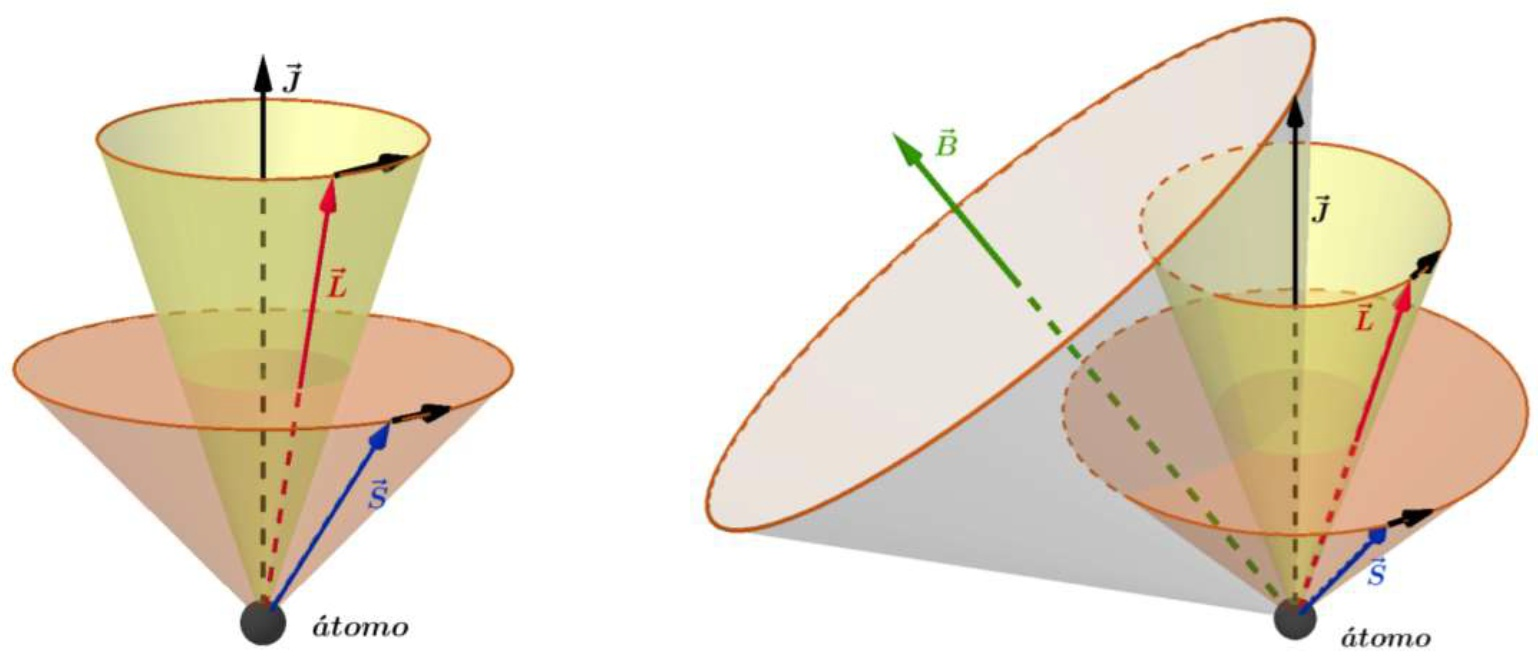
\includegraphics[width=1.0\textwidth]{./Figures/fig116}
	\caption{Interacción L-S}
	\label{fig:116}
 \end{figure}


\section{Momento magnético total de un átomo libre}

El momento magnético efectivo del átomo seria la suma de las componentes $\V{\mu_{L}}$ y $\V{\mu_{S}}$. Calculemos las suma de los momentos magnético que llamamos $\V{\mu_{total}}$

\begin{sloppypar}
\begin{equation}
	\V{\mu}_{total}=\V{\mu}_{L}+\V{\mu}_{S}=-\mu_{B}(\V{L}+g\V{S})=-\mu_{B}(\V{L}+2\V{S})=-\mu_{B}(\V{J}+\V{S})
\end{equation}

Esta expresión nos indica que $\mu_{total}$ es directamente opuesto a $\V{J}$, salvo que ${\V{S}=0}$, $\V{\mu}_{total}$ también girará alrededor de $\V{J}$. La componente de $\mu_{total}$ en la dirección de $\V{J}$ es $\V{\mu_{j}}$ Como se observa en la figura \ref{fig:117}, en la cual no se respetaron las longitudes relativas de los vectores.

\begin{figure}[H]
    \centering
    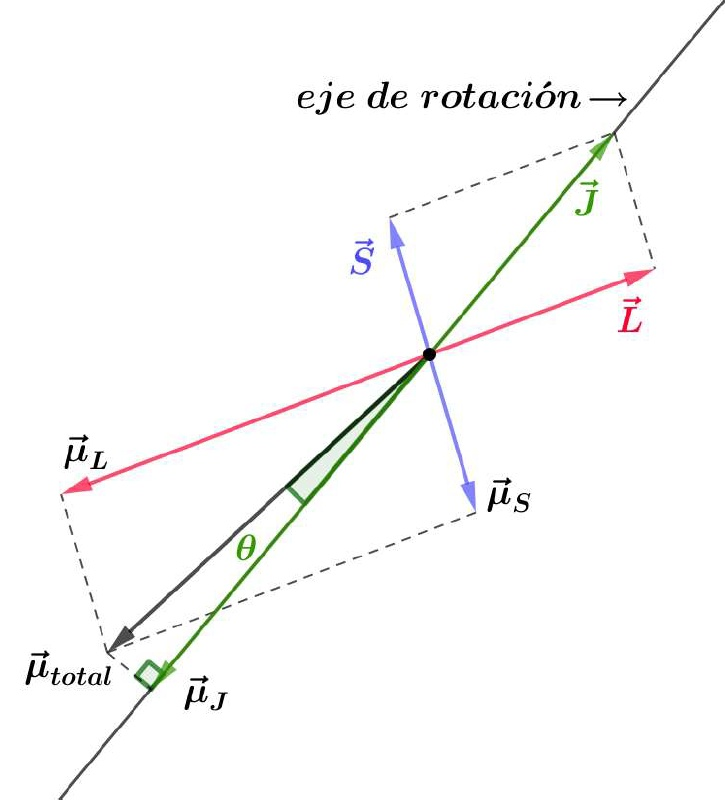
\includegraphics[width=0.7\textwidth]{./Figures/fig117}
	\caption{Momento magnético total de un átomo libre II}
	\label{fig:117}
 \end{figure}

\end{sloppypar}


\begin{itemize}


\item Anteriormente se vio que el momento angular orbital y de espín se sumaban formando el momento magnético atómico total. El momento magnético total de un átomo libre tiene tres contribuciones el momento magnético del núcleo, el momento magnético orbital más el momento magnético del electrón

\item El núcleo atómico tiene carga y presenta momento magnético, este eses103veces inferior a los generados por los electrones, luego, \textbf{no se considera el momento magnético nuclear}.

\item Luego en un átomo, el campo magnético observado es debido al acoplamiento de estos dos momentos: \textbf{orbital y del espín}. 
\end{itemize}

Como sabemos el momento angular total $\V{J}$ es la suma del momento del spin $\V{S}$ con el orbital $\V{L}$. El momento magnético en la dirección $\hat{J}$ será:

\begin{equation}
	\mu_{j}=\lv{\mu_{j}}=\lv{\mu_{l}}Cos(\beta)+\lv{\mu_{s}}Cos(\alpha)
\end{equation}

Donde el ángulo $\hat{SJ}= \alpha$ y el ángulo $\hat{LJ}=\beta$, reemplazando y operando se llega a:

\begin{equation*}
	\mu_{j}=g_{j}\mu_{B}\sqrt{\qa{j}} \quad \text{con } g_{j} \text{ factor de Landé para } j \text{que vale: }
\end{equation*}

\begin{equation*}
	g_{j}= 1 +\dfrac{\qa{l}+\qa{s}-\qa{l}}{2\qa{j}} \quad \text{como veremos seguidamente}
\end{equation*}

Como sabemos el $\mu_{total}$ no esta en la dirección de $\V{J}$ y recordando que $\V{L}$ y $\V{S}$ rotan alrededor de $\V{J}$, luego $\V{\mu}_{L}$ y $\V{L}_{S}$  también rotal alrededor de $\V{J}$. En el esquema se observa la distribución espacial de los mismos. Luego si pretendemos sumarlos es adecuado descomponer $\V{\mu}_{S}$ y $\V{\mu}_{S}$ en dos componentes, una en la dirección del eje de rotación y la otra perpendicular al mismo, esta ultima, como rota, tendrá valor medio cero. Por el contrario, si tendrá un valor determinado distinto de cero, aquellas que proyectamos en la dirección del eje de rotación.


\begin{figure}[H]
    \centering
    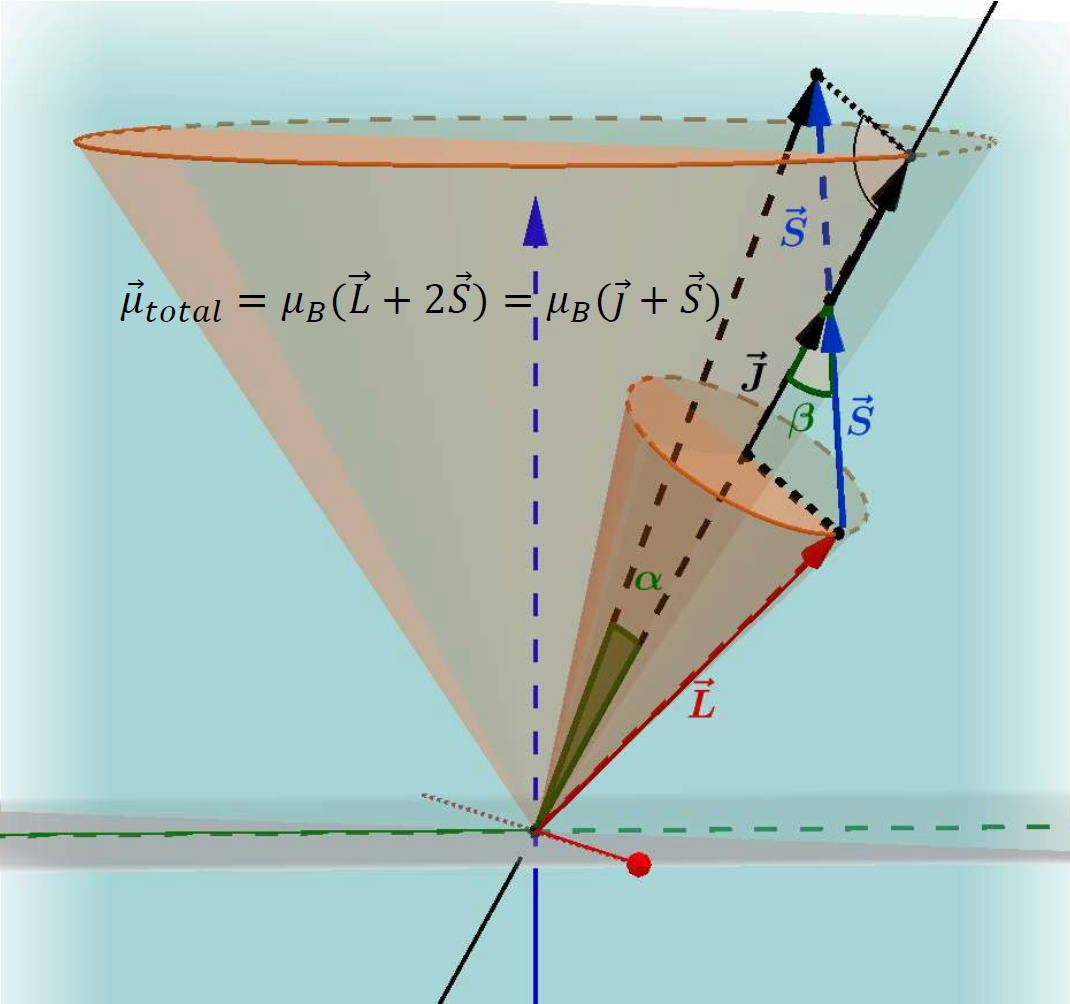
\includegraphics[width=0.9\textwidth]{./Figures/fig118}
	\caption{Momento magnético total de un átomo libre II}
	\label{fig:118}
 \end{figure}

En la figura \ref{fig:119} se observan los ángulos que se utilizaran en el desarrollo de $g_{e}$ como veremos a continuación

\begin{figure}[H]
    \centering
    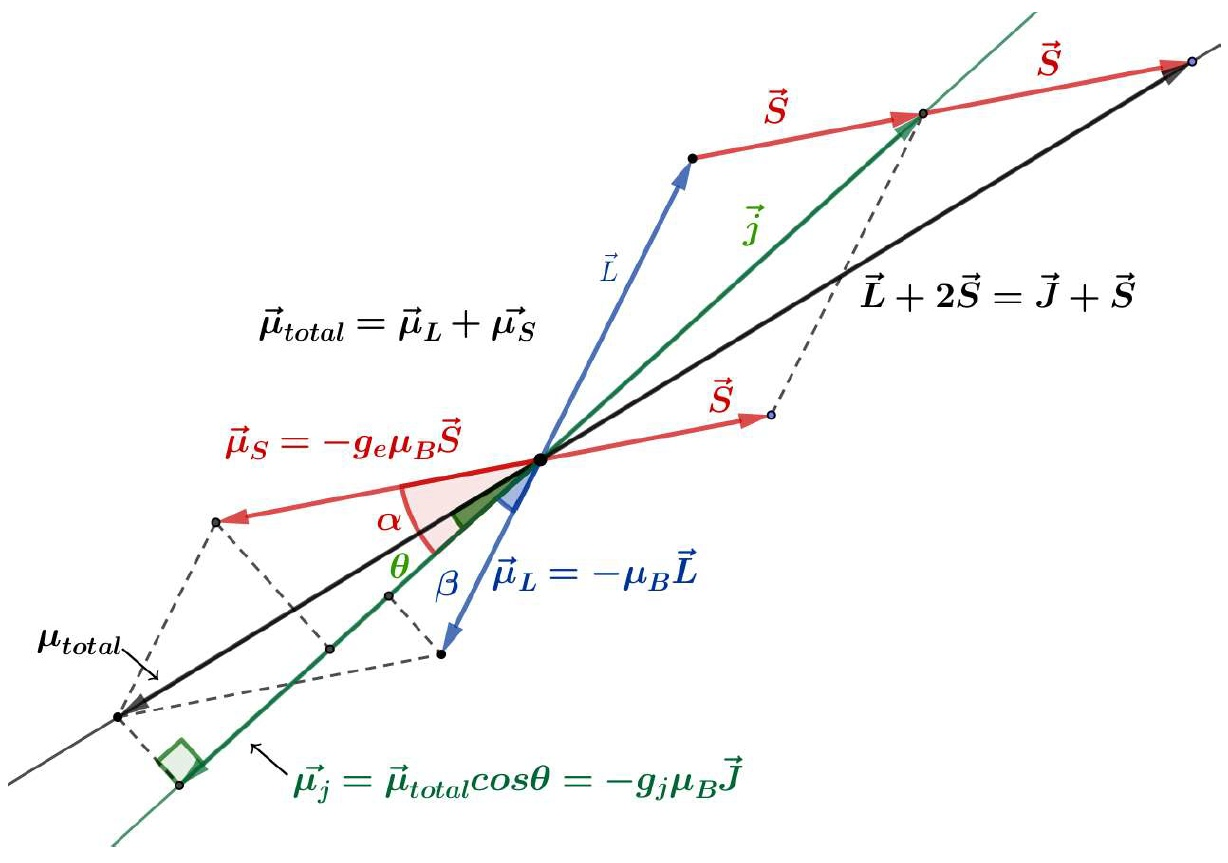
\includegraphics[width=1.0\textwidth]{./Figures/fig119}
	\caption{Momento magnético total de un átomo libre III}
	\label{fig:119}
 \end{figure}
 
Dijimos que:
 
\begin{equation*}
	\mu_{j}=\lv{\mu_{j}}=\lv{\mu_{l}}Cos(\beta)+\lv{\mu_{s}}Cos(\alpha)
\end{equation*} 

y por el teorema del coseno:

\begin{equation*}
	\begin{aligned}[c]
	&\lv{S}^{2}=\lv{L}^{2}+\lv{J}^{2}-2\lv{L}\lv{J}Cos(\beta)\therefore \\
	&Cos(\beta)=\dfrac{\lv{L}^{2}+\lv{J}^{2}-\lv{S}^{2}}{2\lv{L}\lv{J}}= \dfrac{\qa{l}+\qa{j}-\qa{s}}{2\sqrt{\qa{l}\qa{j}}}
	\end{aligned}
\end{equation*} 

De igual manera procedemos para el otro triangulo:

\begin{equation*}
Cos(\alpha)= \dfrac{\qa{s}+\qa{j}-\qa{l}}{2\sqrt{\qa{s}\qa{j}}}
\end{equation*} 

Remplazando los cosenos en la ecuación:

\begin{equation*}
	\begin{aligned}[c]
	&\lv{\mu_{j}}=\lv{\mu_{l}}Cos(\beta)+\lv{\mu_{s}}Cos(\alpha) \\
	&\lv{\mu_{j}}=\lv{\mu_{l}}\dfrac{\qa{l}+\qa{j}-\qa{s}}{2\sqrt{\qa{l}\qa{j}}}+\lv{\mu_{s}}\dfrac{\qa{s}+\qa{j}-\qa{l}}{2\sqrt{\qa{s}\qa{j}}} \\
	&\lv{\mu_{j}}=\mu_{B}\left[\lv{L} \dfrac{\qa{l}+\qa{j}-\qa{s}}{2\sqrt{\qa{l}\qa{j}}}+2\lv{S}\dfrac{\qa{s}+\qa{j}-\qa{l}}{2\sqrt{\qa{s}\qa{j}}}\right] \\ 
	&\lv{\mu_{j}}=\mu_{B}\left[ \dfrac{\qa{l}+\qa{j}-\qa{s}}{2\sqrt{\qa{j}}}+2\dfrac{\qa{s}+\qa{j}-\qa{l}}{2\sqrt{\qa{j}}}\right] \\
	&\lv{\mu_{j}}=\mu_{B}\left[ \dfrac{3\qa{j}+\qa{s}-\qa{l}}{2\sqrt{\qa{j}}} \right] \\
	&\lv{\mu_{j}}=\mu_{B}\left[ \dfrac{3\qa{j}+\qa{s}-\qa{l}}{2\qa{j}} \right]\sqrt{ \qa{j}} \\	
	&\lv{\mu_{j}}=\mu_{B}\left[1+ \dfrac{\qa{j}+\qa{s}-\qa{l}}{2\qa{j}} \right]\sqrt{\qa{j}} \\	
	&\lv{\mu_{j}}=\mu_{B}\,g_{j}\,\sqrt{\qa{j}}\quad \text{o bien: } \quad \V{\mu}_{j}=\mu_{B}\,g_{j}\,\V{L} 	
	\end{aligned}
\end{equation*} 



\section{Átomos con más de un electrón}
Hemos avanzado bastante con el magnetismo atómico nos faltaría generalizar las ideas a átomos con más de un electrón. Los átomos que nos interesan desde el punto de vista del magnetismo son llamados elementos de transición y poseen gran cantidad de electrones. No se puede resolver teóricamente el sistema de varios cuerpos, ni siquiera en mecánica clásica. Sin embargo es posible, con las ideas expuestas anteriormente, comprender y explicar varios fenómenos de átomos con varios electrones. O sea el estado del electrón en el átomo lo determinan cuatro números cuánticos.


Visto lo expuesto, podríamos preguntarnos:

\textbf{¿Cómo se distribuyen los electrones en los átomos dando origen a los distintos elementos químicos que conforman la tabla periódica?}

Analicemos lo que ya sabemos:

\begin{itemize}
	\item El movimiento de pequeñas partículas (electrones, neutrones, etc.) en una zona limitada del espacio, (pozo de potencial, átomo, molécula) está determinado por parámetros adimensionales llamados números cuánticos, estos pueden tomar determinados valores. La cantidad de números cuánticos necesarios en la solución de un problema depende del número de grados de libertad de la partícula, (pozo de potencial uní dimensional un número cuántico, si el pozo es tridimensional serán tres los números). Si además la partícula puede girar sobre si misma tendremos un número cuántico más.
	\item A distintos valores de los número cuánticos corresponde diferentes energías, luego hay niveles discretos de energía. La partícula no puede tener cualquier energía.
	\item Recordemos que lo mencionada hasta aquí se encuentra justificado experimentalmente y teóricamente. Al resolver el problema del movimiento de un electrón en un átomo en el espacio es necesario introducir tres números cuánticos: $n, l, m_{l}$.
	\item  \textcolor{red}{\textbf{n: Número cuántico principal}} vale 1,2,3….define el tamaño de las orbitas, es el que tiene mayor influencia en la energía, cuando mayor sea mayor será el volumen. Siendo $K (n=1), L(n=2)$.
	\item \textcolor{red}{\textbf{l: Número cuántico del momento angular}} indica la forma del orbital y el momento angular, toma vale $0 ,1, 2,.. (n -1)$. Designando $l=0$ como $s$, $l=1$ como $p$, $l=3$ como $d$, etc.
	\item  \textcolor{red}{\textbf{$\boldsymbol{m_{l}}$: Número cuántico magnético}} define la orientación espacial del orbital frente a un campo magnético externo, toma valores $-l,..,0,..,l$.
	\item \textcolor{red}{\textbf{$\boldsymbol{m_{s}}$: Numero cuántico de espín}} Por último es necesario introducir un cuarto numero cuántico no previsto por la mecánica clásica, el número cuántico de espín toma valores $-\frac{1}{2}$ y $+\frac{1}{2}$ para indicar las dos orientaciones del electrón.
\end{itemize}

Para poder realizar el llenado de las capas electrónicas\footnote{El nombre de Capa Electrónica se deriva del modelo de Bohr, en el cual se postulaba que los grupos de electrones orbitaban el núcleo a ciertas distancias, así que sus órbitas formaban capas alrededor de los núcleos. Las capas electrónicas son numeradas correlativamente, partiendo de la más cercana al núcleo, y se identifican mediante letras: n = 1 capa K, n = 2 capa L, n = 3 capa M,...., n = 7 capa Q,} que se corresponden a cada número cuántico principal n de todos los elementos, debemos introducir algunas ideas más.

\begin{itemize}
	\item \textbf{Principio de Pauli}: en un átomo no puede haber dos electrones con los cuatro números cuánticos iguales.
	
Ya comentamos que en la mecánica clásica y en la cuántica las partículas admiten comportamientos totalmente distintos. En mecánica clásica las partícula se mueven en trayectorias bien determinadas, de tal manera que podemos distinguir una de otra y saber en que instante se encontrara en una dada posición. En cuántica es totalmente distinta la situación. Las partículas idénticas son totalmente indistinguibles. Esto quiere decir, de otra forma, que si en cuántica cambio una partícula por otra igual, el estado cuántico no debe modificarse. Si indicamos con $\Psi(1,2)$ la función de onda de un sistema donde $1$ y $2$ son las coordenadas de la primera y segunda partícula. Si intercambiamos las posiciones de las partículas el sistema sigue descripto por la misma función de onda, al menos multiplicada por una constante $\varepsilon$

\begin{equation*}
	\Psi(1,2)=\varepsilon\Psi(2,1)
\end{equation*}

El valor de $\varepsilon$ viene determinado solo por el tipo de partícula, puede tomar solo dos valores $\varepsilon=+1$ o $\varepsilon=-1$ 

Todas las partículas con espín nulo o entero son llamadas Bosones y cumplen con que:

\begin{equation*}
	\Psi(1,2)=+\Psi(2,1)
\end{equation*}


todas las partículas que tienen spin semientero son llamadad Fermiones y cumplen con que:

\begin{equation*}
	\Psi(1,2)=-\Psi(2,1)
\end{equation*}

Los electrones son Fermiones. La mecánica cuántica impone estrictas leyes sociales (cuando interactúan entre ellas). Por ejemplo los Fermiones en sociedad deben cumplir que no pueden haber dos de ellos en un átomo con el mismo conjunto número cuántico. Esto es el principio de Pauli y fue demostrado a posteriori. Como vemos los fermiones son entes ermitaños, no les gustan sus semejantes, sin embargo son todos iguales, indistinguibles.	
	
	\item \textbf{Regla de Hund\footnote{Reglas de Hund: El estado fundamental de un átomo (estado de más baja energía)viene determinado por la combinación de los números cuánticos de los electrones individuales de la capa incompleta, de acuerdo con un conjunto de instrucciones denominadas reglas de Hund que proporcionan el nº cuántico compuesto J correspondiente al estado fundamental:
\begin{itemize}	
\item[1] Los spines de los electrones se distribuyen de tal manera que exista el mayor número de spines paralelos sin que se viole el principio de Pauli. Haciendo $s = +1/2$ ó $-1/24$ se calcula $Sc$ \textbf{momento angular de espín combinado}.
\item[2] Los electrones con espines combinados según 1. se distribuyen entre los posibles valores de $ml$ de manera que $Sml = Lc$ sea máxima. $Lc$ es el \textbf{momento angular orbital combinado}.
\item[3] Los estados de un átomo, caracterizados por su \textbf{momento angular total $J$}, vienen dados por un número cuántico $J$ que toma valores enteros desde $|Lc - Sc|$ hasta $|Lc + Sc|$. El estado fundamental viene dado por $J = |Lc - Sc|$ para una capa llena hasta menos de la mitad, y $J= |Lc + Sc|$ para una capa llena hasta más de la mitad.
\end{itemize}}}: Al llenar orbitales, los tres $p$, los cinco $d$ o los siete $f$ , de igual capa nivel de energía o capa n, los electrones se distribuyen, siempre que sea posible, con sus espines paralelos (apuntando en la misma dirección), ya que la partícula es más estable (tiene menos energía) cuando tiene electrones desapareados (espines paralelos) que cuando esos electrones están apareados (espines opuestos o antiparalelos)
\end{itemize}

Podemos imaginar que los átomos que constituyen la tabla periódica se van formando agregando electrones, estos crean nuevos orbítales una vez que se llenan los primeros. O sea si $n=1$ y $l=0$ es la primer capa que se llena con dos electrones, $n=2$ tenemos dos sub capas una para $n=1$ y $l=0$ estamos en el caso anterior, si $l=1$ tenemos dos subcapas, en total 8 electrones, siguiendo de esta manera obtenemos todos los átomos de la tabla periódica. La repetición de $l$ corresponde a  propiedades químicas similares, luego los átomos que tengan en su ultima capa un solo electrón en la subcapa $s$ tienen propiedades similares. Veamos algunos elementos y sus estructuras electrónicas $H= 1S^{1}, \; He=1s^{2}, \; Li=1s^{2}2s_{1}, \; Be=1s^{2}2s_{2}$


\begin{figure}[H]
    \centering
    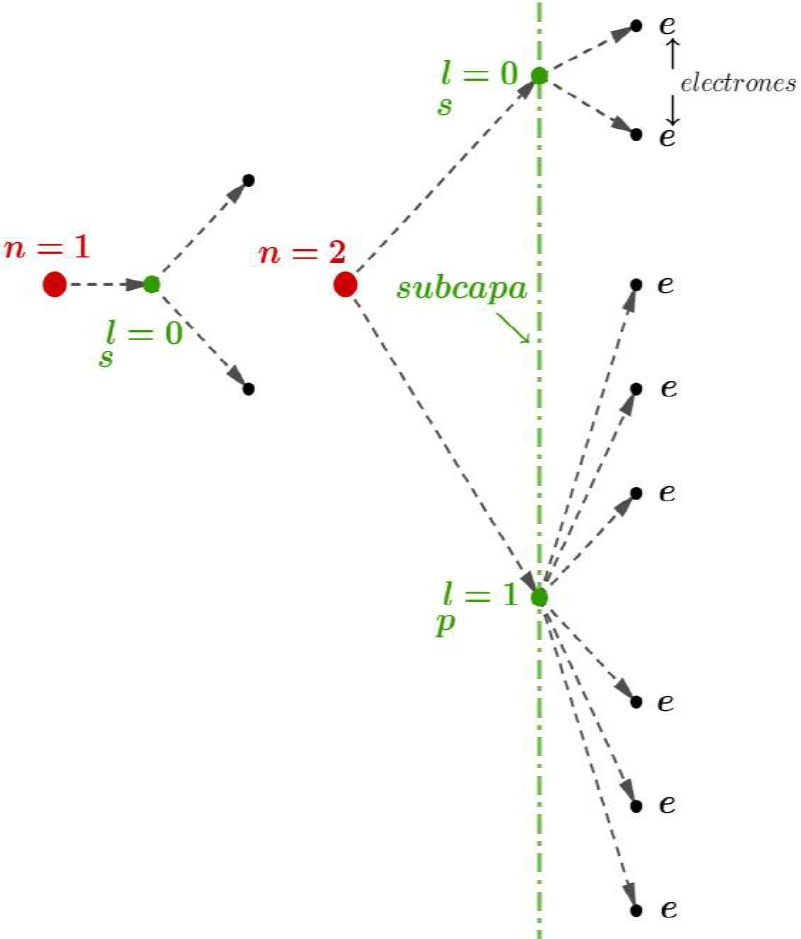
\includegraphics[width=0.8\textwidth]{./Figures/fig120}
	\caption{Distribución de fermiones $e^{-}$}
	\label{fig:120}
 \end{figure}


Los electrones deben cumplir una serie de condiciones para ser introducidos al átomo. Para ello debemos desarrollar la regla empírica de Friedrich Hund presentada en 1927 o de máxima multiplicidad, la cual nos indica como ubicar los electrones. Al llenar orbitales, de igual energía, los electrones se distribuyen, siempre que sea posible, con sus espines paralelos (apuntando en la misma dirección), ya que la partícula es más estable cuando tiene electrones desapareados (spines paralelos) que cuando esos electrones están apareados (spines opuestos o antiparalelos). Dicho de otro modo, se introducen los electrones de tal manera que ocupen primeramente las regiones del átomo donde la probabilidad de encontrarlos en el espacio es mayor. Veamos en el esquema un caso real y otro imposible. Existen varias reglas para ir llenando los orbitales, regla de \textit{Aufbau} es una de ellas. La palabra \textit{aufbau} se refiere al verbo alemán “construir“ no es el nombre de ningún científico

\begin{figure}[H]
    \centering
    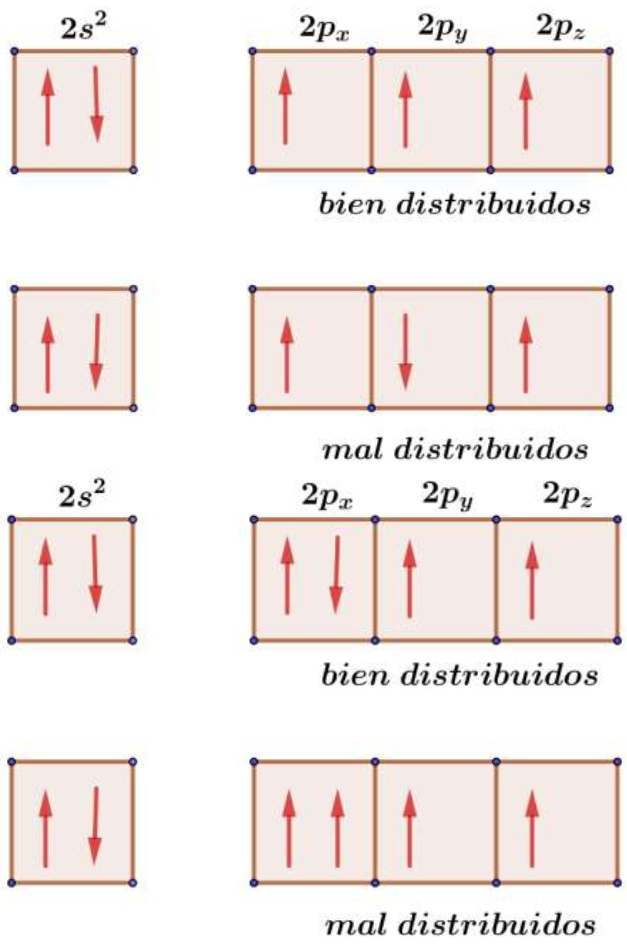
\includegraphics[width=0.4\textwidth]{./Figures/fig121}
	\caption{Distribución siguiendo la regla de Hund}
	\label{fig:121}
 \end{figure}

Al ir agregando electrones obtenemos la tabla periódica de los elementos. Vemos que el primer grupo se inicia con el $H$ y finaliza con $He$ que llena la capa $1s$ con dos electrones y es noble. Luego, el siguiente nivel $n$ comienza con el $Li$ se llena la capa $2s$ con el $Be$ y se completa la capa $2p$ con el $Ne$ que también es noble. La capa siguiente es similar. Podemos verlo en la figura \ref{fig:122}


\begin{figure}[H]
    \centering
    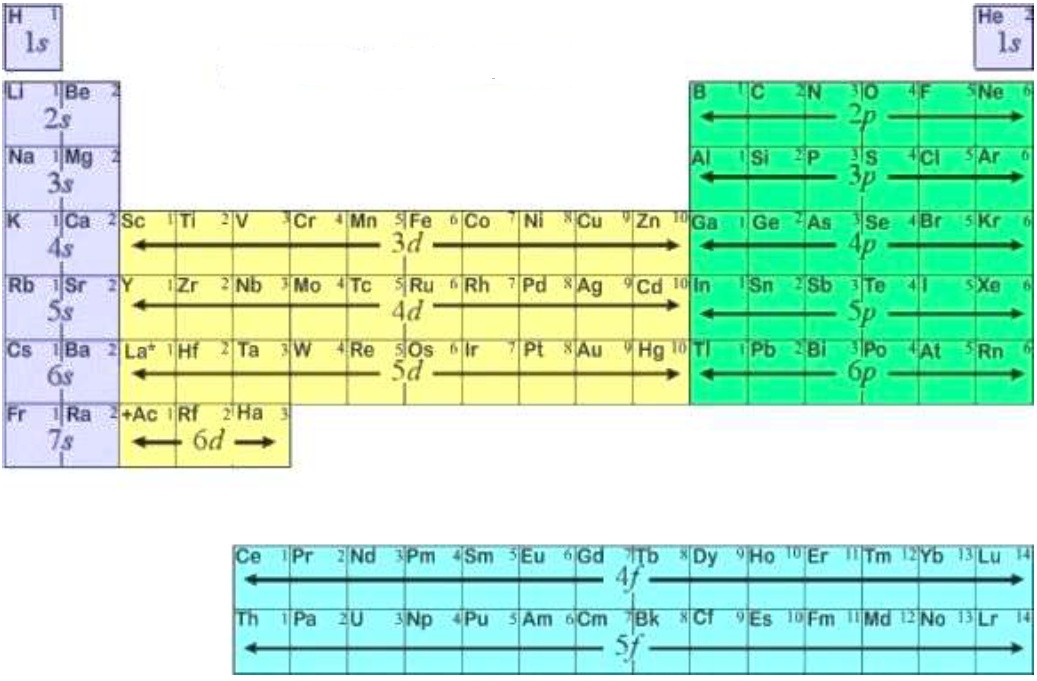
\includegraphics[width=1.0\textwidth]{./Figures/fig122}
	\caption{Capas $n$ y orbitales $l$}
	\label{fig:122}
 \end{figure}

Si los electrones llenan por completa la capa $n$ o $l$ prefijada, tienen momento orbital total y de espín nulo, por ejemplo los gases inertes $He,\; Ne,\; Ar,\; Kr,\; Xe\; \text{y}\; Rn$  La mayoría de los átomos tienen un momento magnético distinto de cero como podemos ver en la tabla de la figura \ref{fig:GraficoAlineaciónDelSpin}


\begin{figure}[H]
    \centering
    \includegraphics[width=1.0\textwidth]{./Figures/AlineaciónDelSpin}
	\caption{Alineación de los espines electrónicos}
	\label{fig:GraficoAlineaciónDelSpin}
\end{figure}


\textbf{Recordando algo de química:}

Cada capa se compone de una o más subcapas, que a su vez se componen de los orbitales atómicos. Por ejemplo, la primera capa ($K$) tiene una subcapa, llamada $1s$; la segunda capa ($L$) tiene dos subniveles, llamados $2s$ y $2p$; la tercera capa ($M$) tiene $3s$, $3p$ y $3d$; la cuarta ($N$) tiene las subcapas $4s$, $4p$, $4d4$ y $4f4$; la quinta capa ($O$) tiene $5s$, $5p$, $5d$ y $5f$ etc.

\begin{figure}[H]
    \centering
    \includegraphics[width=0.6\textwidth]{./Figures/Gráfico5}
	\caption{Llenado de los orbitales,}
	\label{fig:Grafico5}
\end{figure}

en la figura \ref{fig:Grafico5} podemos observar que de $3p$ se pasa a $4s$. El potasio comienza a llenar la $4s$, sin haber completado la $3d$.

El número cuántico $l$ determina la excentricidad de la órbita, cuando mayor sea, más excéntrica será.
Así para todos los $l=0$ ($1s$, $2s$, $3s$, etc.) independientemente de la capa, tendremos un orbital esférico.

\begin{figure}[H]
    \centering
    \includegraphics[width=0.6\textwidth]{./Figures/1S2S3S}
	\caption{orbitales esféricos de las capas s}
	\label{fig:Grafico1s2s3s}
\end{figure}

A partir de la capa $L (n=2)$, corresponderá además de $l=0$, $l= 1$ ($2p$, $3p$, $4p$, etc.)


\begin{figure}[H]
    \centering
    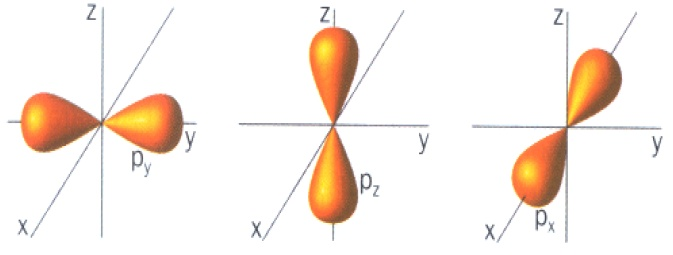
\includegraphics[width=0.8\textwidth]{./Figures/OrbitalesP}
	\caption{orbitales p}
	\label{fig:GraficoOrbitalesP}
\end{figure}

\begin{figure}[H]
    \centering
    \includegraphics[width=0.6\textwidth]{./Figures/Gráfico7}
	\caption{orbitales l}
	\label{fig:Grafico7}
\end{figure}

Podemos ver como se acomodan las primeras capas y orbitales:

\begin{figure}[H]
    \centering
    \includegraphics[width=0.7\textwidth]{./Figures/variosOrbitales}
	\caption{orbitales sucesivos}
	\label{fig:variosOrbitales}
\end{figure}

Con la capa $M$ ($n=3$) comienzan los orbitales $d$, $l=2$: $3d$, $4d$, $5d$, etc.

\begin{figure}[H]
    \centering
    \includegraphics[width=0.8\textwidth]{./Figures/Gráfico8}
	\caption{orbitales d}
	\label{fig:Grafico8}
\end{figure}








\subsection{Suma de momentos angulares o momento angular total}

Habiamos visto para el átomo con un solo electrón que podíamos suponer que los dos momento angulares, el orbital y el de espín, si bien distintos, interactuaban acoplándose, dando origen al momento angular total del átomo (sin el núcleo) que llamamos $\V{J}$ y definimos como $\V{J}=\V{L}+\V{S}$, que debe cumplir las mismas propiedades que los momentos angulares $\V{L}$ y $\V{S}$. Es decir debe ser realizado de acuerdo a los lineamientos de la mecánica cuántica. Este tema suele introducirce como la suma de dos vectores cuantizados $\V{J_{1}}$ y $\V{J_{2}}$. para dar de esta manera generalidad al método. Luego tendremos:


\begin{equation}
	\mid\V{J_{1}}\mid =\sqrt{j_{1}\big(j_{1}+1\big)}\,\hbar \quad \text{con} \quad j_{1z}= m_{1}\hbar \quad \text{y} \quad -j_{1} \leq m_{1} \leq j_{1}
\end{equation}

\begin{equation}
	\mid\V{J_{2}}\mid =\sqrt{j_{2}\big(j_{2}+1\big)}\,\hbar \quad \text{con} \quad j_{2z}= m_{2}\hbar \quad \text{y} \quad -j_{2} \leq m_{2} \leq j_{2}
\end{equation}

%

Donde $j_{1}$ y $j_{2}$ son los números cuánticos correspondientes pudiendo ser enteros o semi enteros

\begin{equation}
	j_{1} \quad \text{y} \quad j_{2} \; \in \; \lbrace 0,\, \frac{1}{2},\, 1,\, \frac{3}{2},\, 2,\, \ldots\, \rbrace
\end{equation}

También $\V{J}=\V{L}+\V{S}$ deberá cumplir con las condiciones que impone la mecánica cuántica a los momento angulares, es decir:

\begin{equation}
	\mid\V{J}\mid =\sqrt{j\big(j+1\big)}\,\hbar \quad \text{con} \quad j_{z}= m\hbar \quad \text{y} \quad -j \leq m \leq j
\end{equation}

El número cuántico del momento angular total puede variar en pasos de a uno entre:

\begin{equation}
	\mid j_{1}-j_{2} \mid \leq j \leq \mid j_{1}+j_{2} \mid
\end{equation}

\subsection{Momento angular total de un átomo}

\begin{itemize}
	\item \textbf{Ejemplo:} supongamos que $\V{J_{1}}=\V{L}$  y $\V{J_{2}}=\V{S}$ , luego $\V{J}=\V{L}+\V{S}$ , como vimos $j$ varia entre $\mid j_{1}-j_{2} \mid \leq j \leq \mid j_{1}+j_{2} \mid$ o sea $\mid l-\frac{1}{2} \mid \leq j \leq \mid l+\frac{1}{2} \mid$, luego $j=l\pm\frac{1}{2}$.
	\item Si $l=0$ entonces $j=\frac{1}{2}$ (estado $s$ se designa $s_{\frac{1}{2}}$).	
	\item Si $l=1$ entonces $j=\frac{1}{2}; j=\frac{3}{2}$ (estado $p$ se designa $p_{\frac{1}{2}}; p_{\frac{3}{2}}$).
	\item Podemos tener una imagen del fenómeno pensando que la suma se realiza de manera clásica, pero, no es tan así. Clásicamente para sumarlos deberíamos conocer el ángulo que forman los vectores y sus módulos, luego aplicar el teorema del coseno.
	\item Sigamos con el ejemplo: vimos que para el caso en que $l\neq0$ el momento angular total $J=l\pm\frac{1}{2}$, calculemos el modulo de $\mid\V{J}\mid =\sqrt{j\big(j+1\big)}\,\hbar$ para los dos casos del número cuántico $j$ del momento angular total


\begin{figure}[H]
    \centering
    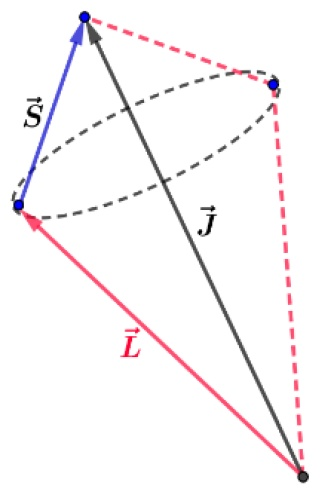
\includegraphics[width=0.4\textwidth]{./Figures/GraficoJLS}
	\caption{Momneto angular total J=L+S}
	\label{fig:GraficoJLS}
\end{figure}



\begin{equation}
	j=\frac{1}{2} ;\quad j=-\frac{1}{2}
\end{equation}	
\end{itemize}

	
Momento angular total de un átomo:
\begin{itemize}
	\item 1. Si:\; $\textcolor{red}{j=l+\frac{1}{2}} \quad\Rightarrow\quad \mid\V{J}\mid =\sqrt{j\big(j+1\big)}\,\hbar = \sqrt{\big(l+\frac{1}{2}\big)\big(l+\frac{3}{2}\big)}\,\hbar$
	\item 2. Si:\; $\textcolor{red}{j=l-\frac{1}{2}} \quad\Rightarrow\quad \mid\V{J}\mid =\sqrt{j\big(j+1\big)}\,\hbar = \sqrt{\big(l+\frac{1}{2}\big)\big(l-\frac{1}{2}\big)}\,\hbar$
\end{itemize}
	
La magnitud del momento angular de espín será:
\begin{equation}
 \mid\overrightarrow{S}\mid =\sqrt{s\big(s+1\big)}\,\hbar = \frac{\sqrt{3}}{2} \quad \text{para} \quad s=\frac{1}{2} 
\end{equation}

De la misma manera se puede obtener los momentos magnético:

%\begin{equation}
\begin{multline}
  \V{\mu}=\V{\mu_{L}}+\V{\mu_{S}}=-\frac{e}{2m}\big(\V{L}+g\,\V{S}\big)=-\frac{e}{2m}\big(\V{L}+2\V{S}\big)=\\
  -\frac{e}{2m}\big(\left[\V{L}+\V{S}\right]+\V{S}\big)= -\frac{e}{2m}\big(\V{J}+\overrightarrow{S}\big)
  \label{eq:uno}
\end{multline}
%\end{equation}

La ecuación (\ref{eq:uno}) nos indica que $\V{\mu}$ no es directamente opuesto a $\V{J}$, salvo que $\V{S} = 0$

Podemos sumar a los vectores $\V{L}$ y $\V{S}$ por que interactúan, si bien mantienen sus orientaciones relativas experimentan una precesión alrededor de $\V{J}$, también precesiona $\V{\mu}$ alrededor de $\V{J}$. La componente de $\V{\mu}$ en la dirección de $\V{j}$ es $\V{\mu_{j}}$. Observemos que hay precesión pese a la ausencia de campo externo al átomo, este fenómeno se llama interacción espín-orbita.

Aquí observamos los gráficos de los dos casos particulares comentados anteriormente, más adelante se ampliara con la interacción $S-L$


\begin{figure}[H]
    \centering
    \includegraphics[width=0.7\textwidth]{./Figures/Gráfico10a}
	\caption{Momento magnético total}
	\label{fig:Grafico10c}
\end{figure}


\begin{figure}[H]
    \centering
    \includegraphics[width=0.7\textwidth]{./Figures/Gráfico10b}
	\caption{Momento magnético total}
	\label{fig:Grafico10c}
\end{figure}


\subsection{Momento magnético total de un átomo}

El momento magnético efectivo del átomo es $\V{\mu_{J}}$, la suma de las componentes $\V{\mu_{L}}$ y $\V{\mu_{S}}$. Si el átomo esta en un campo magnético débil, de tal manera, que no se rompe el acoplamiento entre $\V{L}$ y $\V{S}$ , en este caso $\V{J}$ experimentará una precesión alrededor de $\V{\mu_{H}}$ , el campo exterior.

Esta formulación, que se expone, puede posiblemente ser vista como arbitraria y antojadiza; realmente cobra sentido cuando se ve cómo logra explicar fenómenos experimentales tales como el efecto Zeeman o el experimento de Stern-Gerlach. La realidad es que se crea ad-hoc para explicar estos fenómenos. Nuestro interés es solo comprender el origen del magnetismo

\begin{figure}[H]
    \centering
    \includegraphics[width=0.8\textwidth]{./Figures/Gráfico10c}
	\caption{Momento magnético total}
	\label{fig:Grafico10c}
\end{figure}


\subsubsection{Momento magnético total}

\begin{itemize}
\item Anteriormente se vio que el momento angular orbital y de espín se sumaban formando el momento atómico total. El momento magnético total de un átomo libre tiene tres contribuciones: el momento magnético del núcleo, el momento magnético orbital más el momento magnético del electrón.
\item El núcleo atómico tiene carga y presenta momento magnético, este es $10^3$ veces inferior a los generados por los electrones, luego, no los consideramos en este caso.
\item Luego en un átomo, el campo magnético observado es debido al acoplamiento de estos dos momentos: \textcolor{red}{Orbital} y de \textcolor{red}{Spin}, los cuales generan campos magnéticos y reaccionan ante la presencia de los mismos.
\end{itemize}

Como sabemos el momento angular total $\V{J}$ es la suma del momento del espín $\V{S}$ y el orbital $\V{L}$.

\begin{figure}[H]
    \centering
    \includegraphics[width=0.6\textwidth]{./Figures/Gráfico10d}
	\caption{Momento magnético total átomo libre}
	\label{fig:Grafico10d}
\end{figure}


El momento magnético en la dirección $z$ será:
\begin{equation}
	\mu_{j} = \mu_{zS}+\mu_{zL} = g\,m_{S}\mu_{B}+m_{L}\mu_{B}
\end{equation}

donde las proyecciones se hallan como $\mu_{zS}=\mu_{S}Cos(SJ)$ y $\mu_{zL}+\mu_{L}Cos(LJ)$. Remplazando y operando se llega a:

\begin{equation}
	\mu_{j} = g_{j}\sqrt{j(j+1)}\,\mu_{B} \quad \text{con} \; g_{j}\;  \text{factor de Landé para}\; j    
\end{equation}

\begin{equation}
	g_{j} = 1 + \frac{s(s+1)-l(l+1)+j(j+1)}{2j(j+1)}
\end{equation}

En la figura \ref{fig:Grafico10d} no se tuvieron en cuenta los casos con signos negativos por simplicidad

\subsubsection{Interacción espín-orbita}

\begin{itemize}
	\item La aplicación de un campo magnético externo al átomo produce precesión y divide las líneas espectrales, este fenómeno es llamado efecto Zeeman.
	\item En un átomo los niveles de energía de los electrones son afectados por una interacción interna del átomo, entre el momento magnético del spin y el momento angular orbital. Esta interacción divide las líneas espectrales, en particular en el hidrogeno como se observa en la figura \ref{fig:GraficoInterEspinOrbita}
	\item La interacción spin-orbita es también una interacción con un campo magnético, pero interno, generado por el movimiento orbital del electrón en el propio átomo que llamamos Zeeman interno.
	\item Si se observan las líneas espectrales del hidrogeno con alta resolución, se encuentran que son dobles y poco espaciadas entre sí. Este fenómeno se llama \textbf{estructura fina}.
	\item Cálculos aproximados demuestran que el campo magnético interno sobre el electrón seria de 0,4 Tesla
	\item Si consideramos el momento dipolar del núcleo, de la interacción de este con el momento orbital y con el spin aparecerán subdivisiones mucho más pequeñas, conocidas como \textbf{estructura hiperfina}.
	
\end{itemize}

\begin{figure}[H]
    \centering
    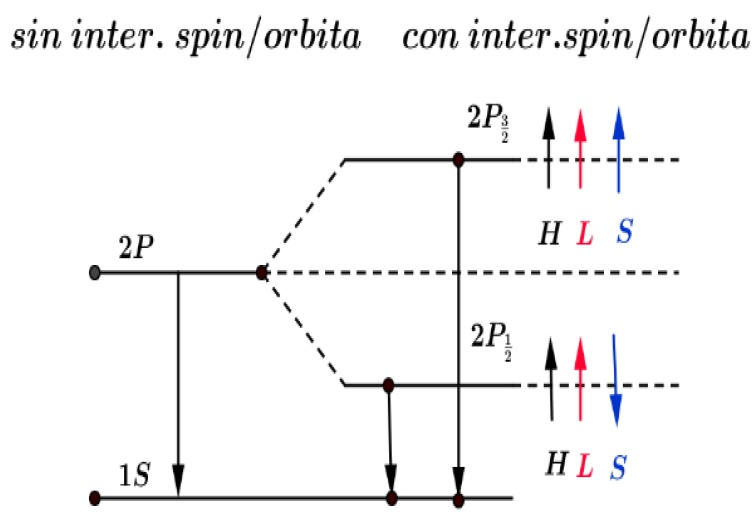
\includegraphics[width=0.6\textwidth]{./Figures/GraficoInterEspinOrbita}
	\caption{Interacción Espín Órbita}
	\label{fig:GraficoInterEspinOrbita}
\end{figure}

La notación $2P\frac{3}{2}$ y $2P\frac{1}{2}$ de la figura \ref{fig:GraficoInterEspinOrbita} es conocida como notación espectroscópica, que no hemos comentado hasta ahora.

\subsection{Átomos con más de un electrón}

El momento angular total de un átomo con más de un electrón es una característica importante por que determina las propiedades magnéticas del átomo.

\textbf{Interacción S-J, Russell-Saunders}
\begin{itemize}
	\item Hay dos formas de sumar los momentos. En los átomos livianos la interacción electrostática es más importante que la magnética, y si los campos magnéticos externos son débiles los espines electrónicos $\V{s_{l}}$ interaccionan entre sí y resultan en un momento angular de espín $\V{S}=\sum_{l}\V{s_{l}}$. Del mismo modo, los momentos angulares orbitales $\V{L_{l}}$ forman el momento angular orbital total $\V{L}=\sum_{l}\V{L_{l}}$. La interacción es llamada de Russell-Saunders, la suma $\V{J}=\sum_{l}(\V{s_{l}}+\V{l_{l}})$ forma el momento angular atómico $\overrightarrow{J}$
\end{itemize}
 
\begin{figure}[H]
    \centering
    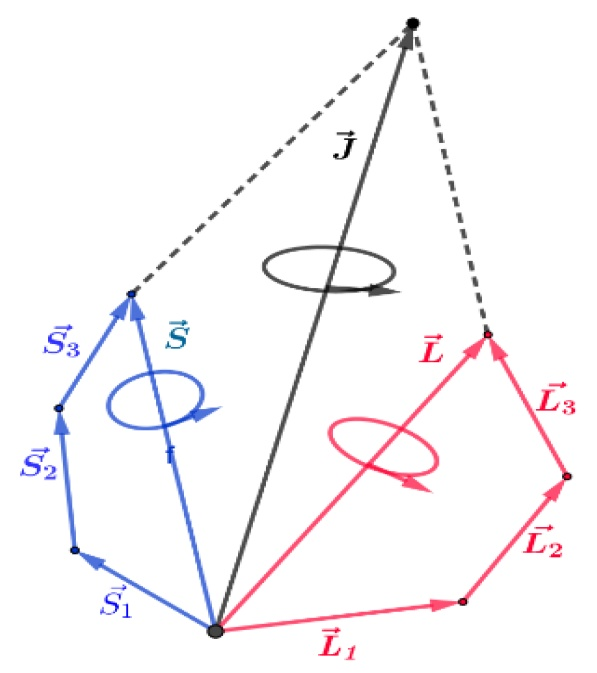
\includegraphics[width=0.6\textwidth]{./Figures/GraficoCaso1}
	\caption{Interacción S-J, Russell-Saunders}
	\label{fig:GraficoCaso1}
\end{figure}

\textbf{Interacción J-J}
\begin{itemize}
	\item Es diferente en los átomos más pesados, donde las interacciones espín-órbita son importantes comparables a las interacciones espín-espín y las órbita-órbita. La interacción $j-j$ es la que prevalece, siendo la opuesta a la Russell-Saunders, y se basa en que la interacción magnética es mucho más importante que la electrostática.
\end{itemize}
 
\begin{figure}[H]
    \centering
    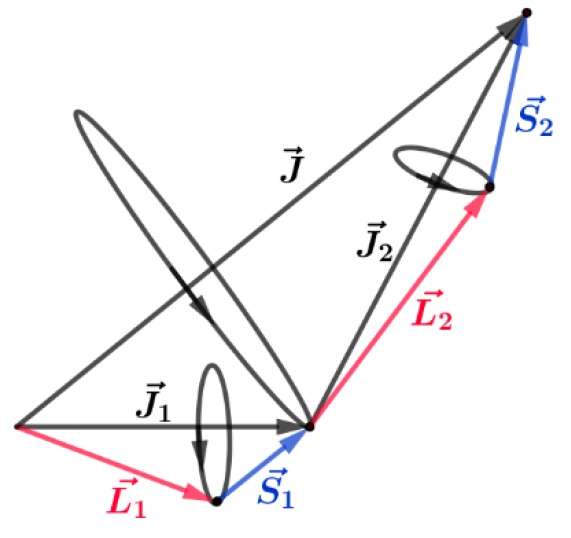
\includegraphics[width=0.6\textwidth]{./Figures/GraficoCaso2}
	\caption{Interacción J-J}
	\label{fig:GraficoCaso2}
\end{figure}

\textbf{Momento orbital bloqueado}
\begin{itemize}
	\item Algo particular sucede en los
elementos de transición. Estos son los que tienen la subcapa $d$ o $f$ parcialmente llena. El término 'elementos de transición' se refiere más comúnmente a los elementos del bloque $d$. El zinc, cadmio y mercurio no cumplen estrictamente con las propiedades de transición. Por lo general son metales de alto punto de fusión. Los elementos de transición del bloque $f$ son conocidos como ''elementos de transición interna''. En los electrones de la serie $3d$ no es posible definir una órbita precisa, debido a las interacciones electrostáticas entre los electrones. Esto estaría indicando una interacción del tipo Russell-Saunders,
\end{itemize}
 
 
\begin{figure}[H]
    \centering
    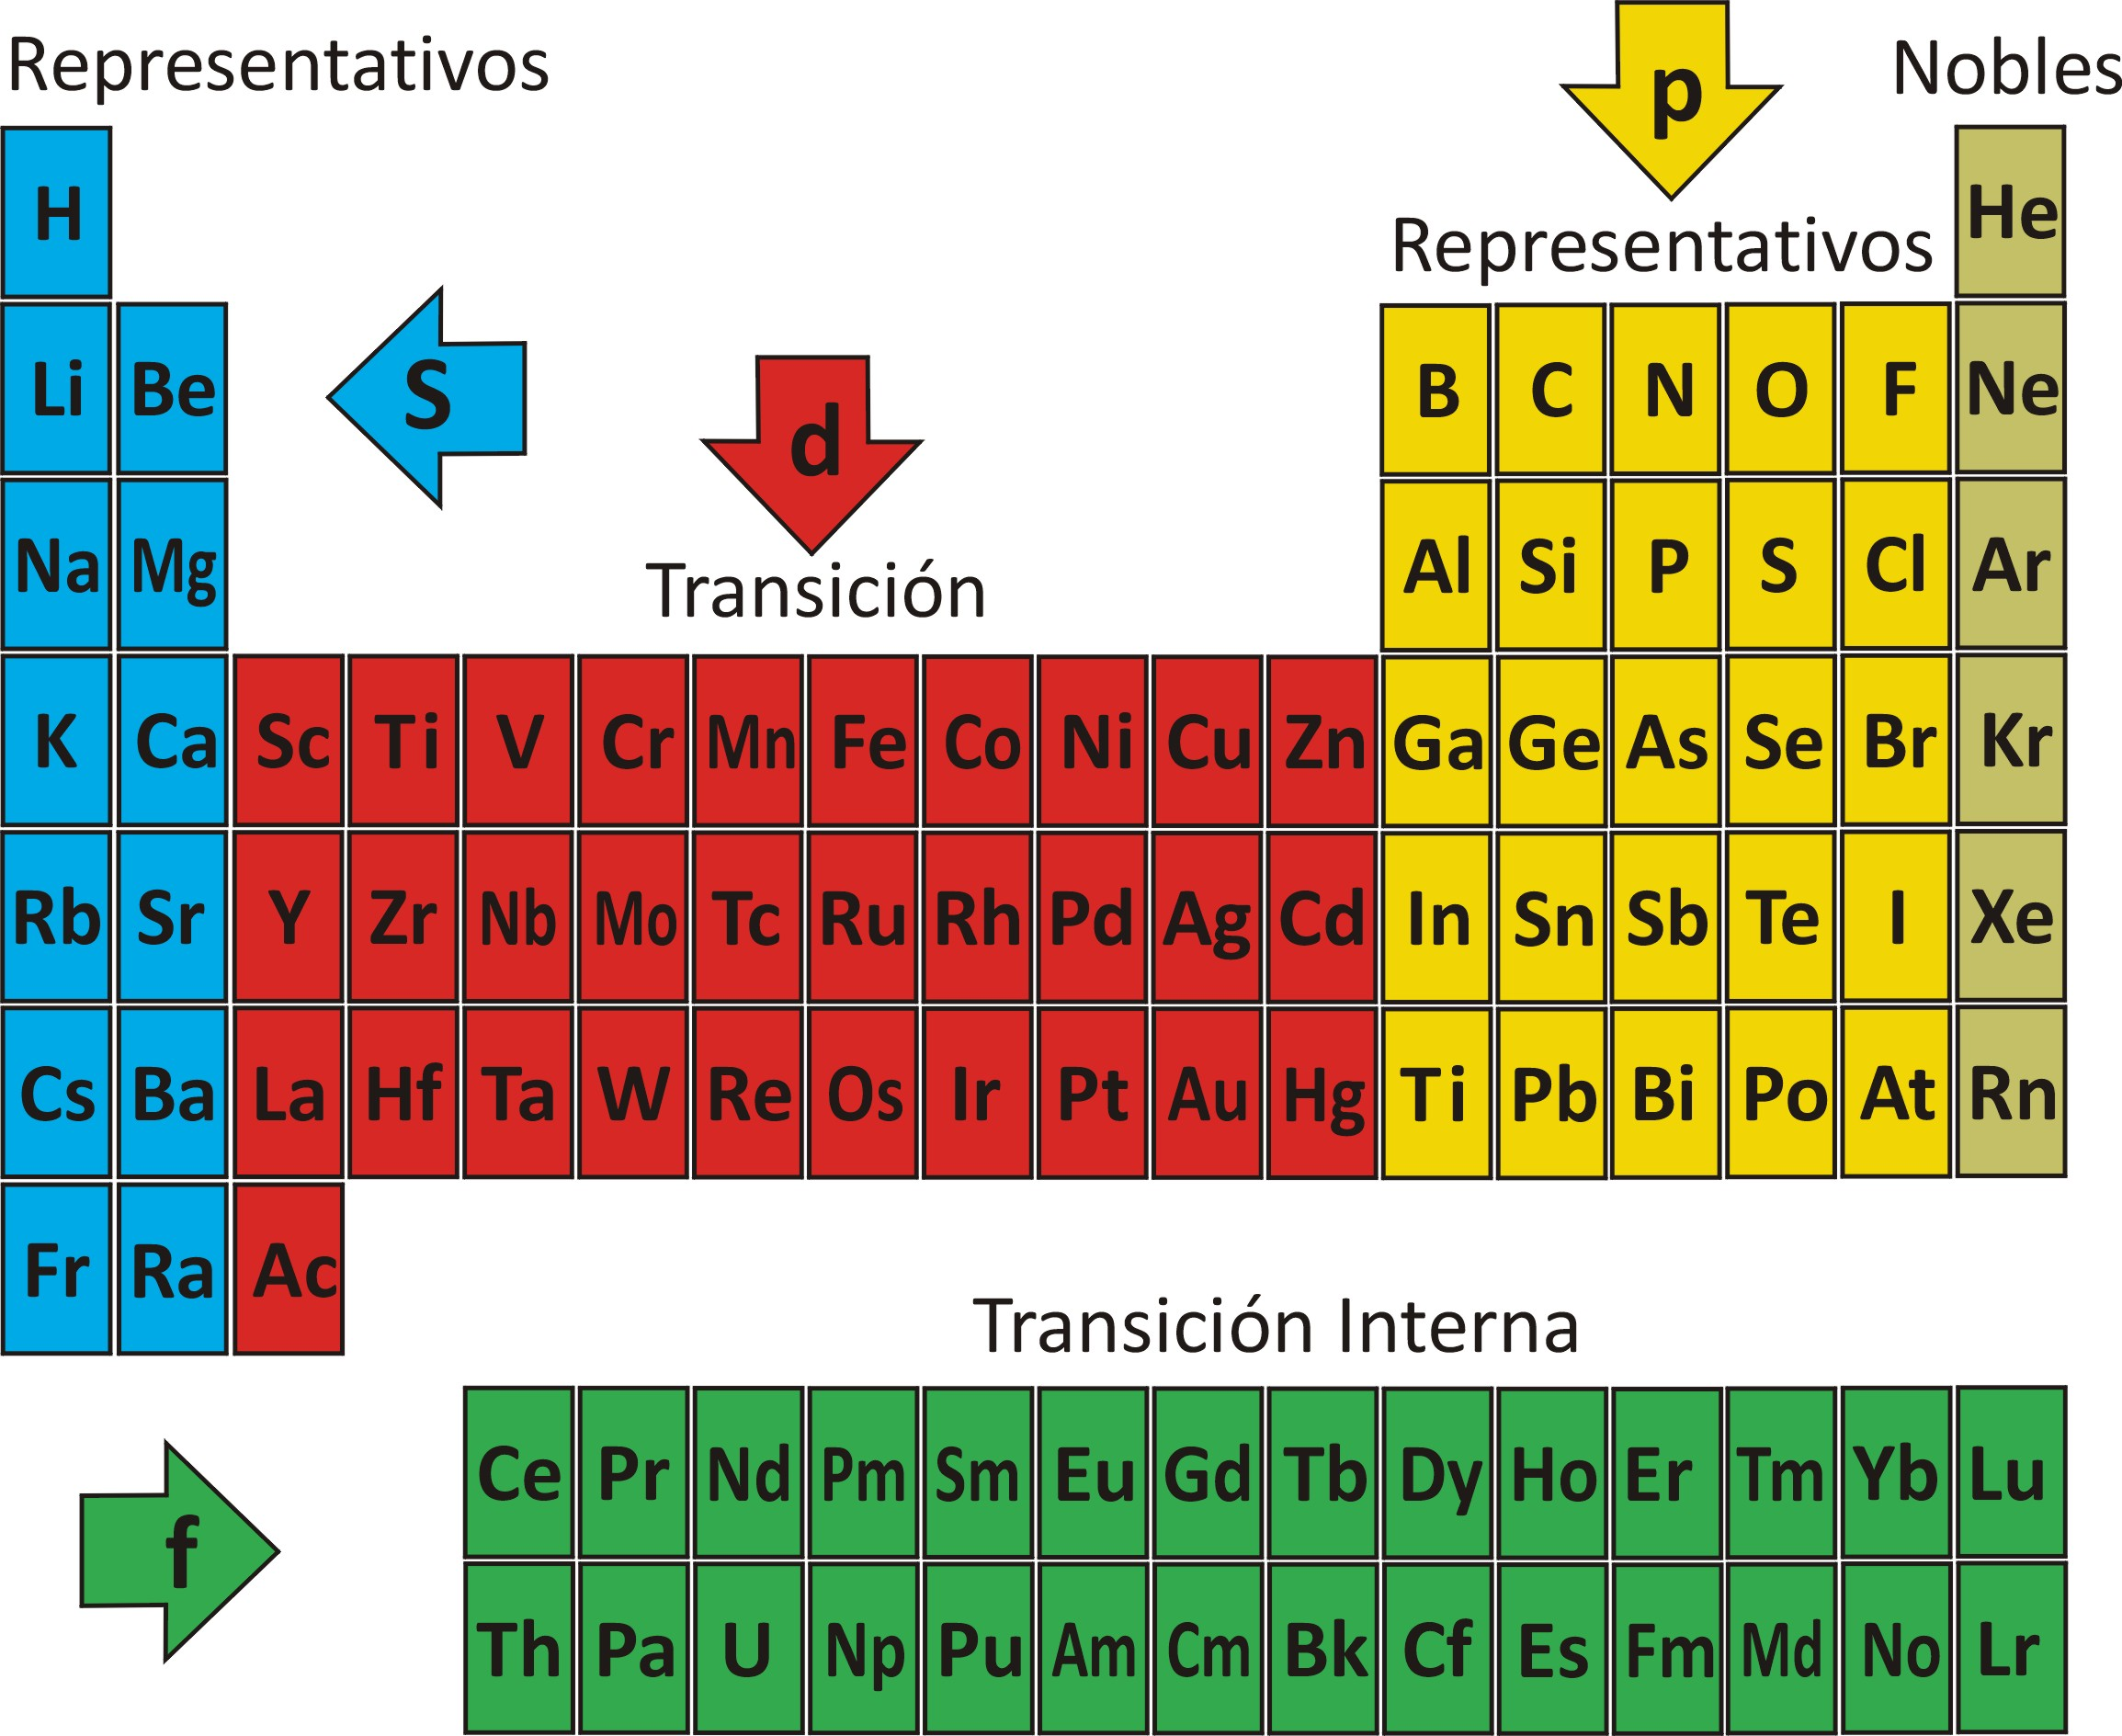
\includegraphics[width=0.8\textwidth]{./Figures/TablaPeriodica}
	\caption{Elementos de transición interna}
	\label{fig:TablaPeriodica}
\end{figure}

luego la suma $\V{J}=\sum_{l}(\V{s_{l}}+\V{l_{l}})$ forma el momento angular atómico $\V{J}$. El momento magnético se calcula $\mu_{j} = g_{j}\sqrt{j(j+1)}\,\mu_B$, sin embargo los resultados experimentales no coinciden con estos
valores y si lo hacen perfectamente con la expresión $g_{s}\sqrt{s(s+1)}\,\mu_B$ como si no existiera el momento orbital. Este fenómeno se expresa diciendo que el momento orbital esta bloqueado y facilita el estudio de los metales que nos interesa.

\textbf{Moraleja: En los metales de transición se considera solo el espín del electrón, (por suerte). Los electrones no apareados les dan las propiedades magnéticas al átomo en el que estén. En tanto en las tierras raras debemos usar el acoplamiento Russell-Sanders.}


Analicemos en particular la configuración electrónica de tres átomos aislados, de
transición de suma importancia en el magnetismo Fe, Ni y Co. Número atómico del Fe= 26, del Ni = 27 y del Co = 28
\vspace{1.0cm}

\begin{figure}[H]
    \centering
    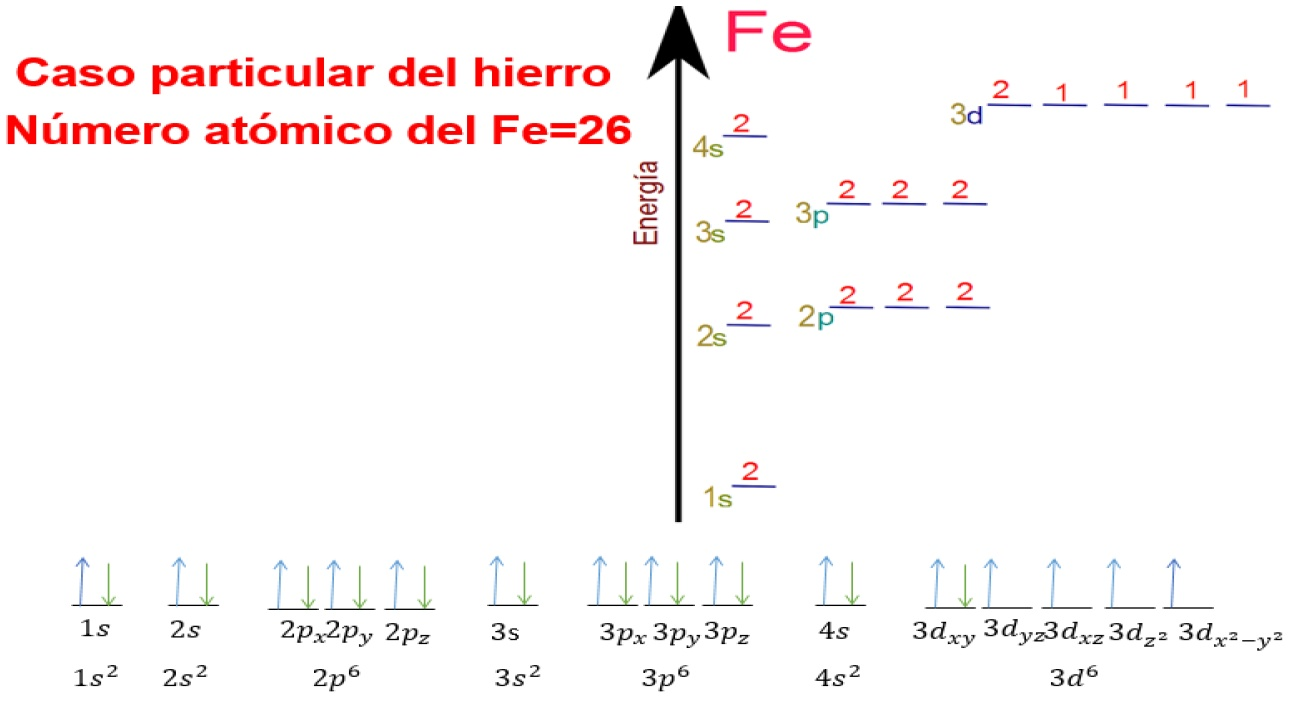
\includegraphics[width=1.0\textwidth]{./Figures/casoDelFe}
	\caption{Distribución electrónica del Hierro}
	\label{fig:casoDelFe}
\end{figure}

\begin{figure}[H]
    \centering
    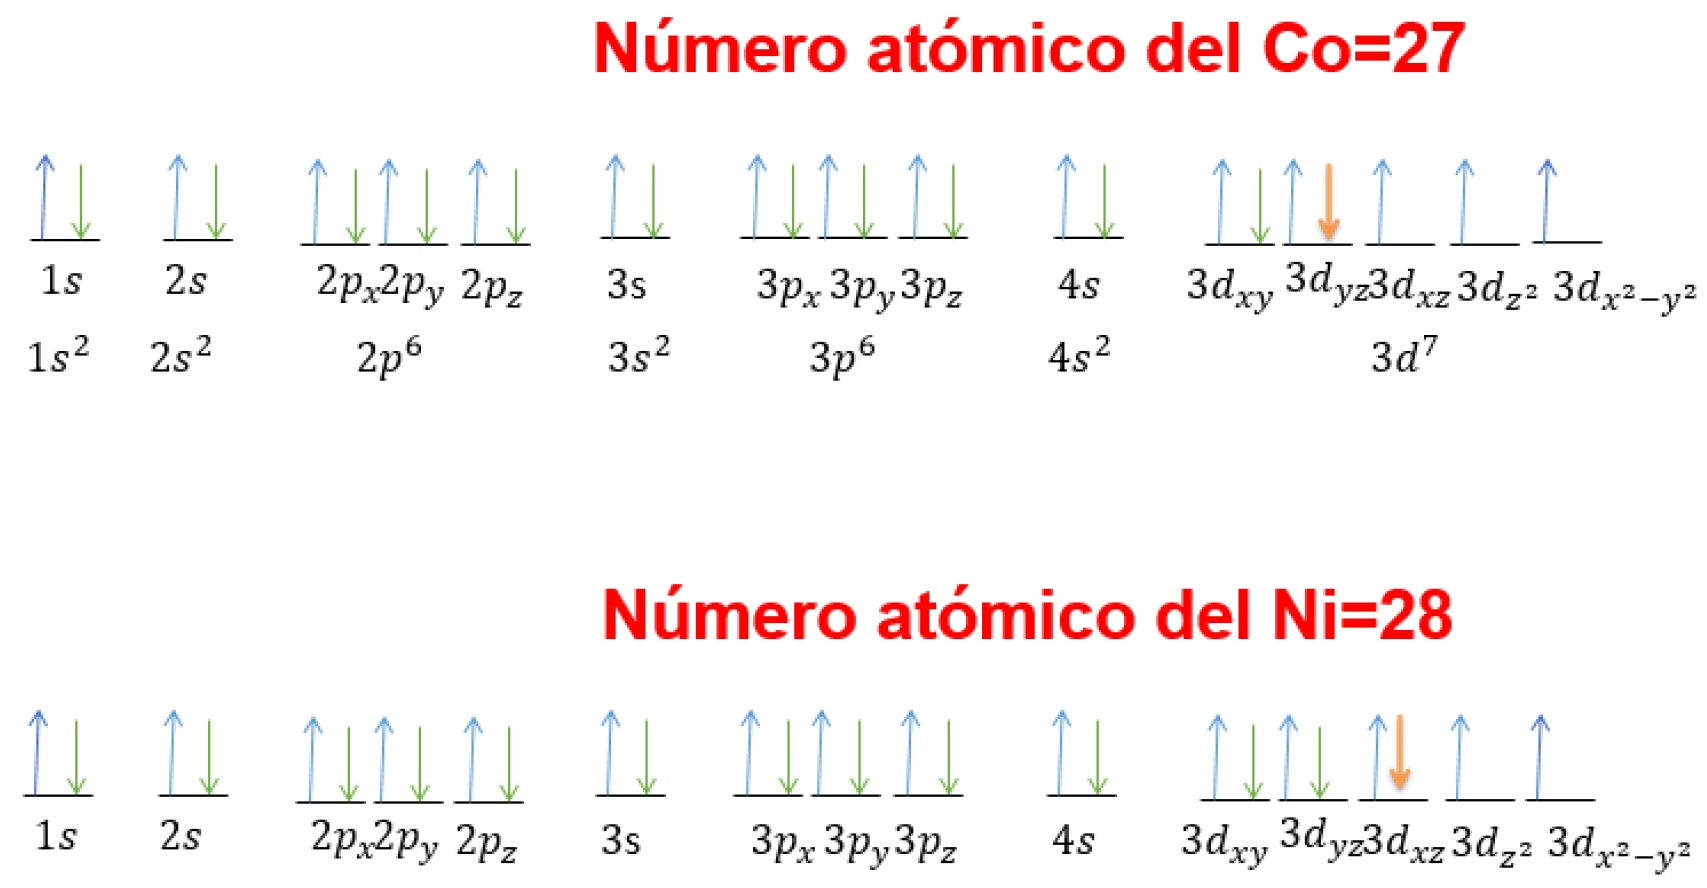
\includegraphics[width=1.0\textwidth]{./Figures/casoDelNiCo}
	\caption{Distribución electrónica del Níquel y el Cobalto}
	\label{fig:casoDelNiCo}
\end{figure}

En la figura \ref{fig:momMagElemTransicion4} vemos la distribución de electrones correspondiente al Fe en distintos estados de oxidación.

\begin{figure}[H]
    \centering
    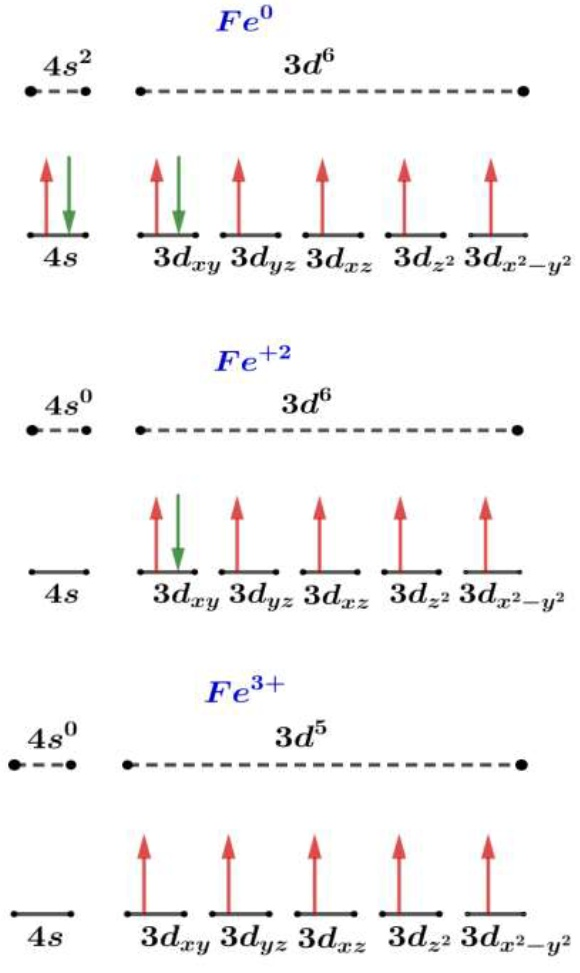
\includegraphics[width=0.6\textwidth]{./Figures/momMagElemTransicion4}
	\caption{Fe en distintos estado de oxidación}
	\label{fig:momMagElemTransicion4}
\end{figure}


\begin{itemize}
	\item Vemos que los átomos con capas externas completas tienen momento magnético cero, (gases inertes pero también Zn, Cd, Hg ), los elementos con solo electrones en la capa $s$ no tienen momento orbital ($l=0$), en estos casos el momento magnético atómico se debe solo al espín. Los alcalinos con un solo electrón en la capa $s$ tienen un momento magnético de un magnetón, lo mismo es cierto para el (Cu, Ag, Au).
	\item Aquellos que tienen una capa interna no completa poseen un momento magnético importante (elementos de transición), estos son los casos que nos interesa. Como ya mencionamos los elementos de transición tienen el momento orbital bloqueado.
\end{itemize}

\subsection{Ejemplos de los grupos 3d y 4f}

Tenemos la estructura $3d^{n} 4s^{2}$ el momento magnético es predominantemente debido al espín, hay poco blindaje de los electrones en el nivel $4s, L\approx0$.


\begin{figure}[H]
    \centering
    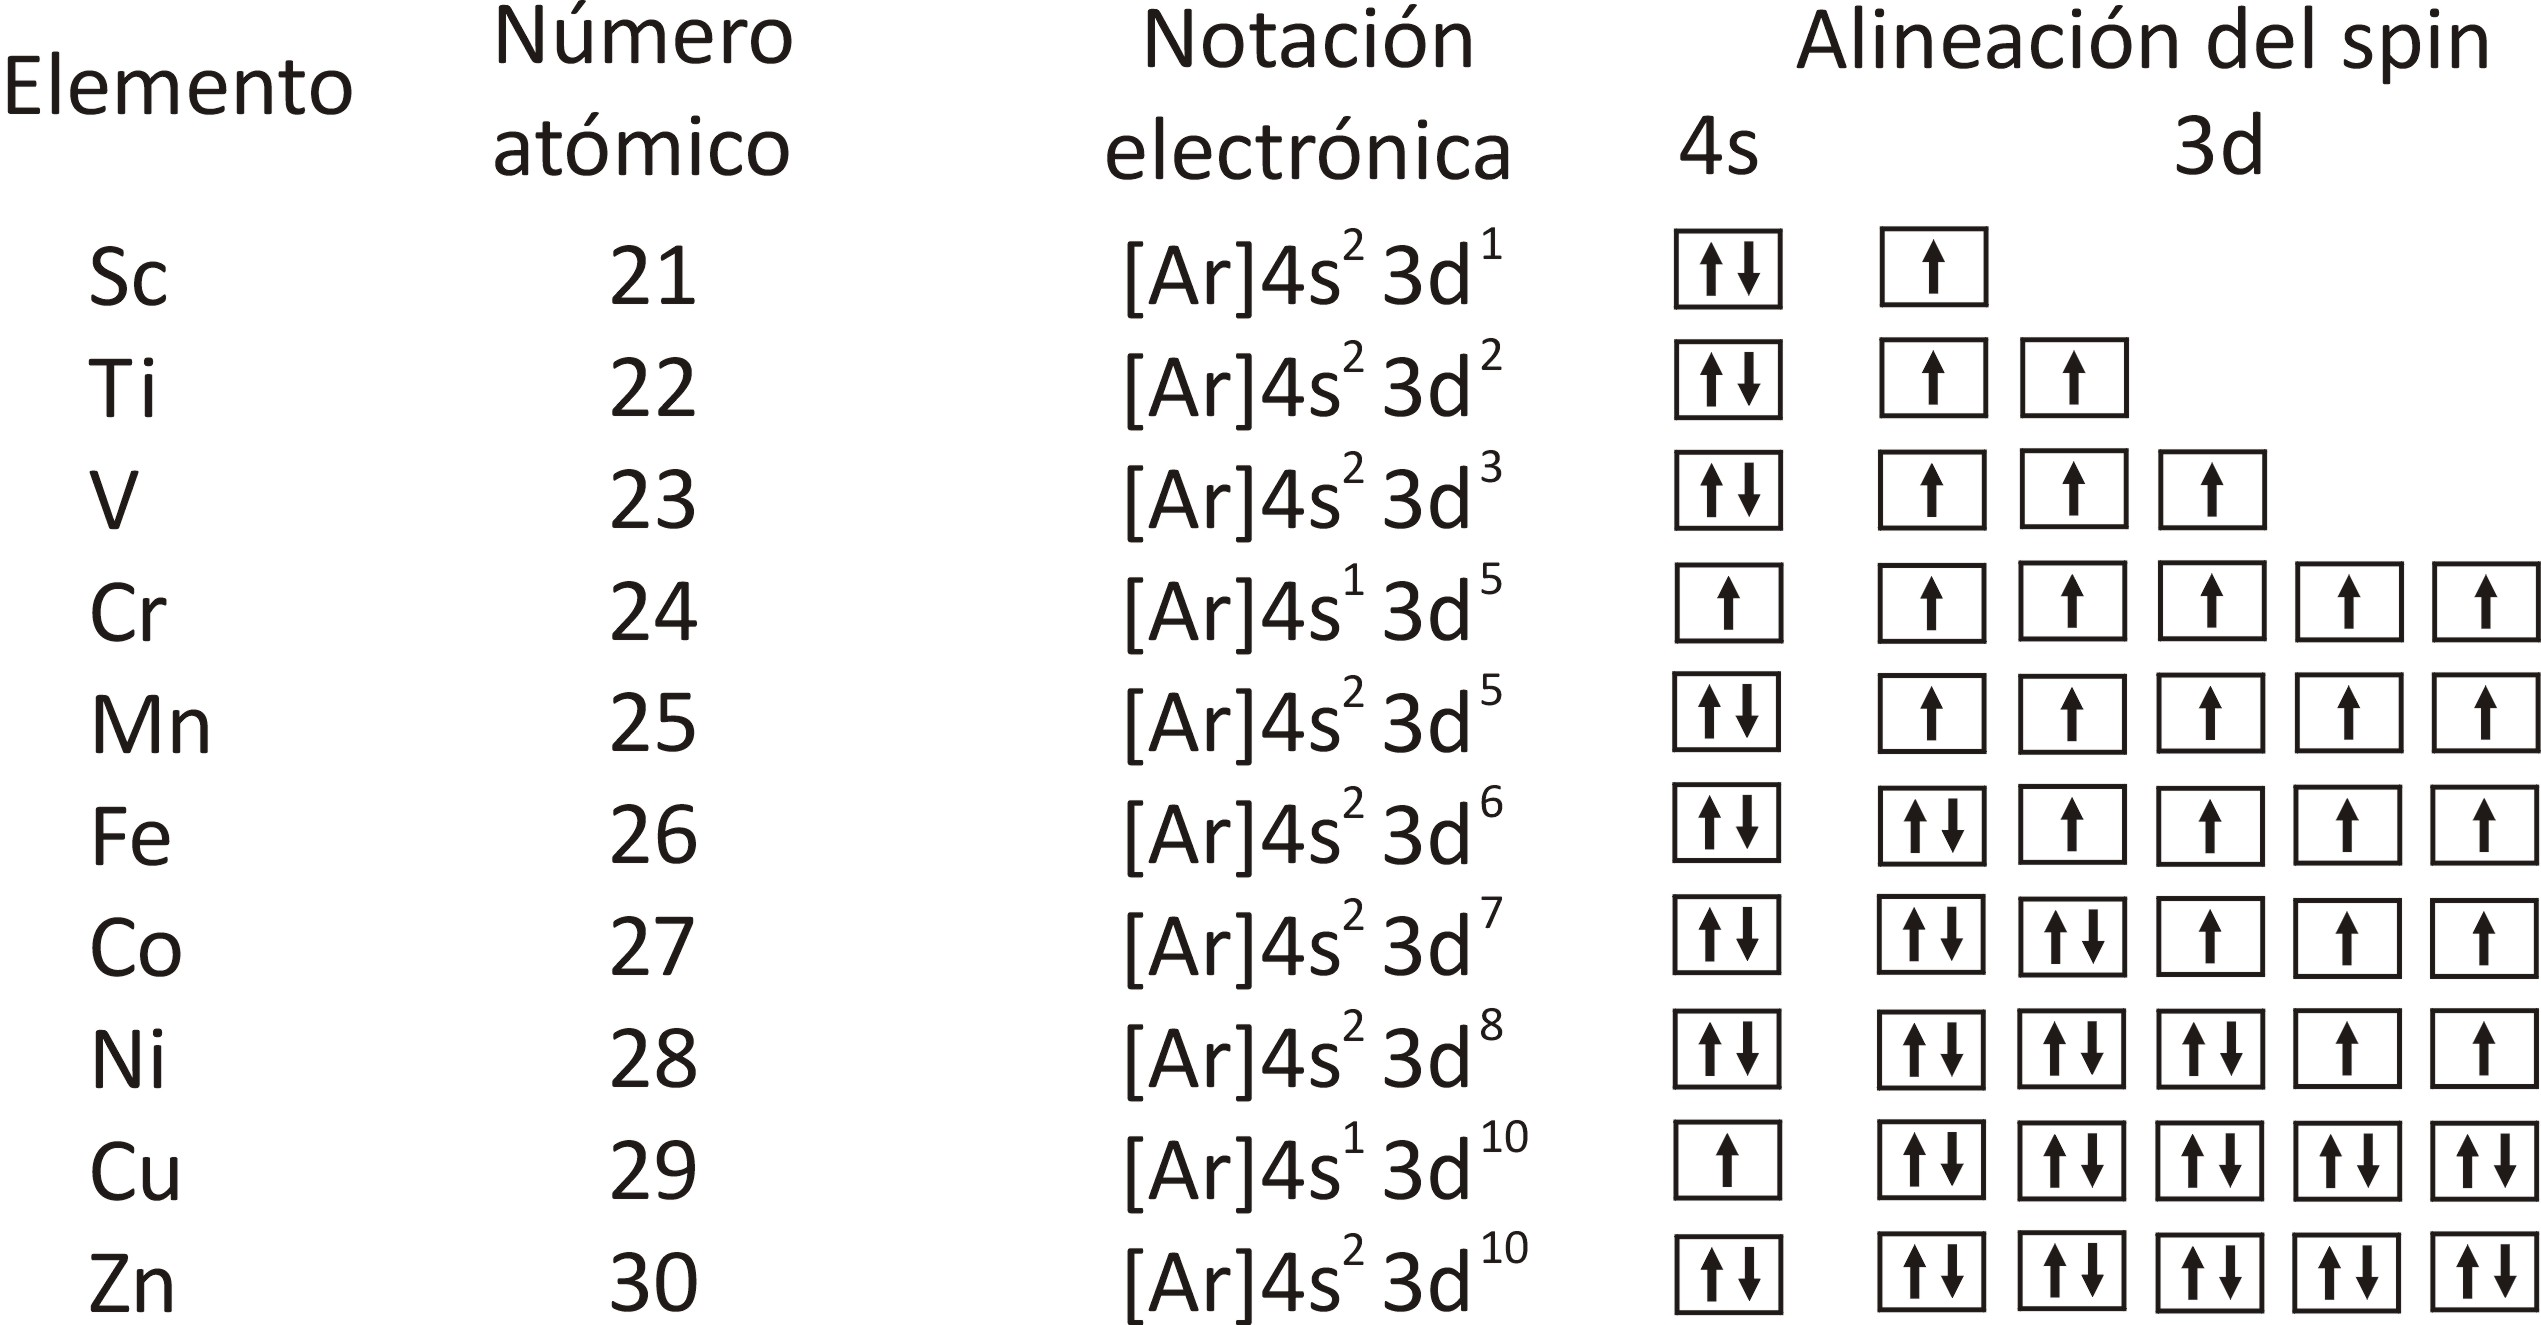
\includegraphics[width=1.0\textwidth]{./Figures/AlineacionDelEspin2}
	\caption{Alineacion del espín grupos 4s 3d}
	\label{fig:AlineacionDelEspin2}
\end{figure}

Tenemos la estructura $4f^{n} 5s^{2} 5p^{6} 6s^{2}$ el momento magnético es predominantemente debido a $L+S$, hay
fuerte blindage de los electrones en los niveles completos $6s\; y\; 5p$. El momento magnético es mayor que el
del grupo $3d$.

\begin{figure}[H]
    \centering
    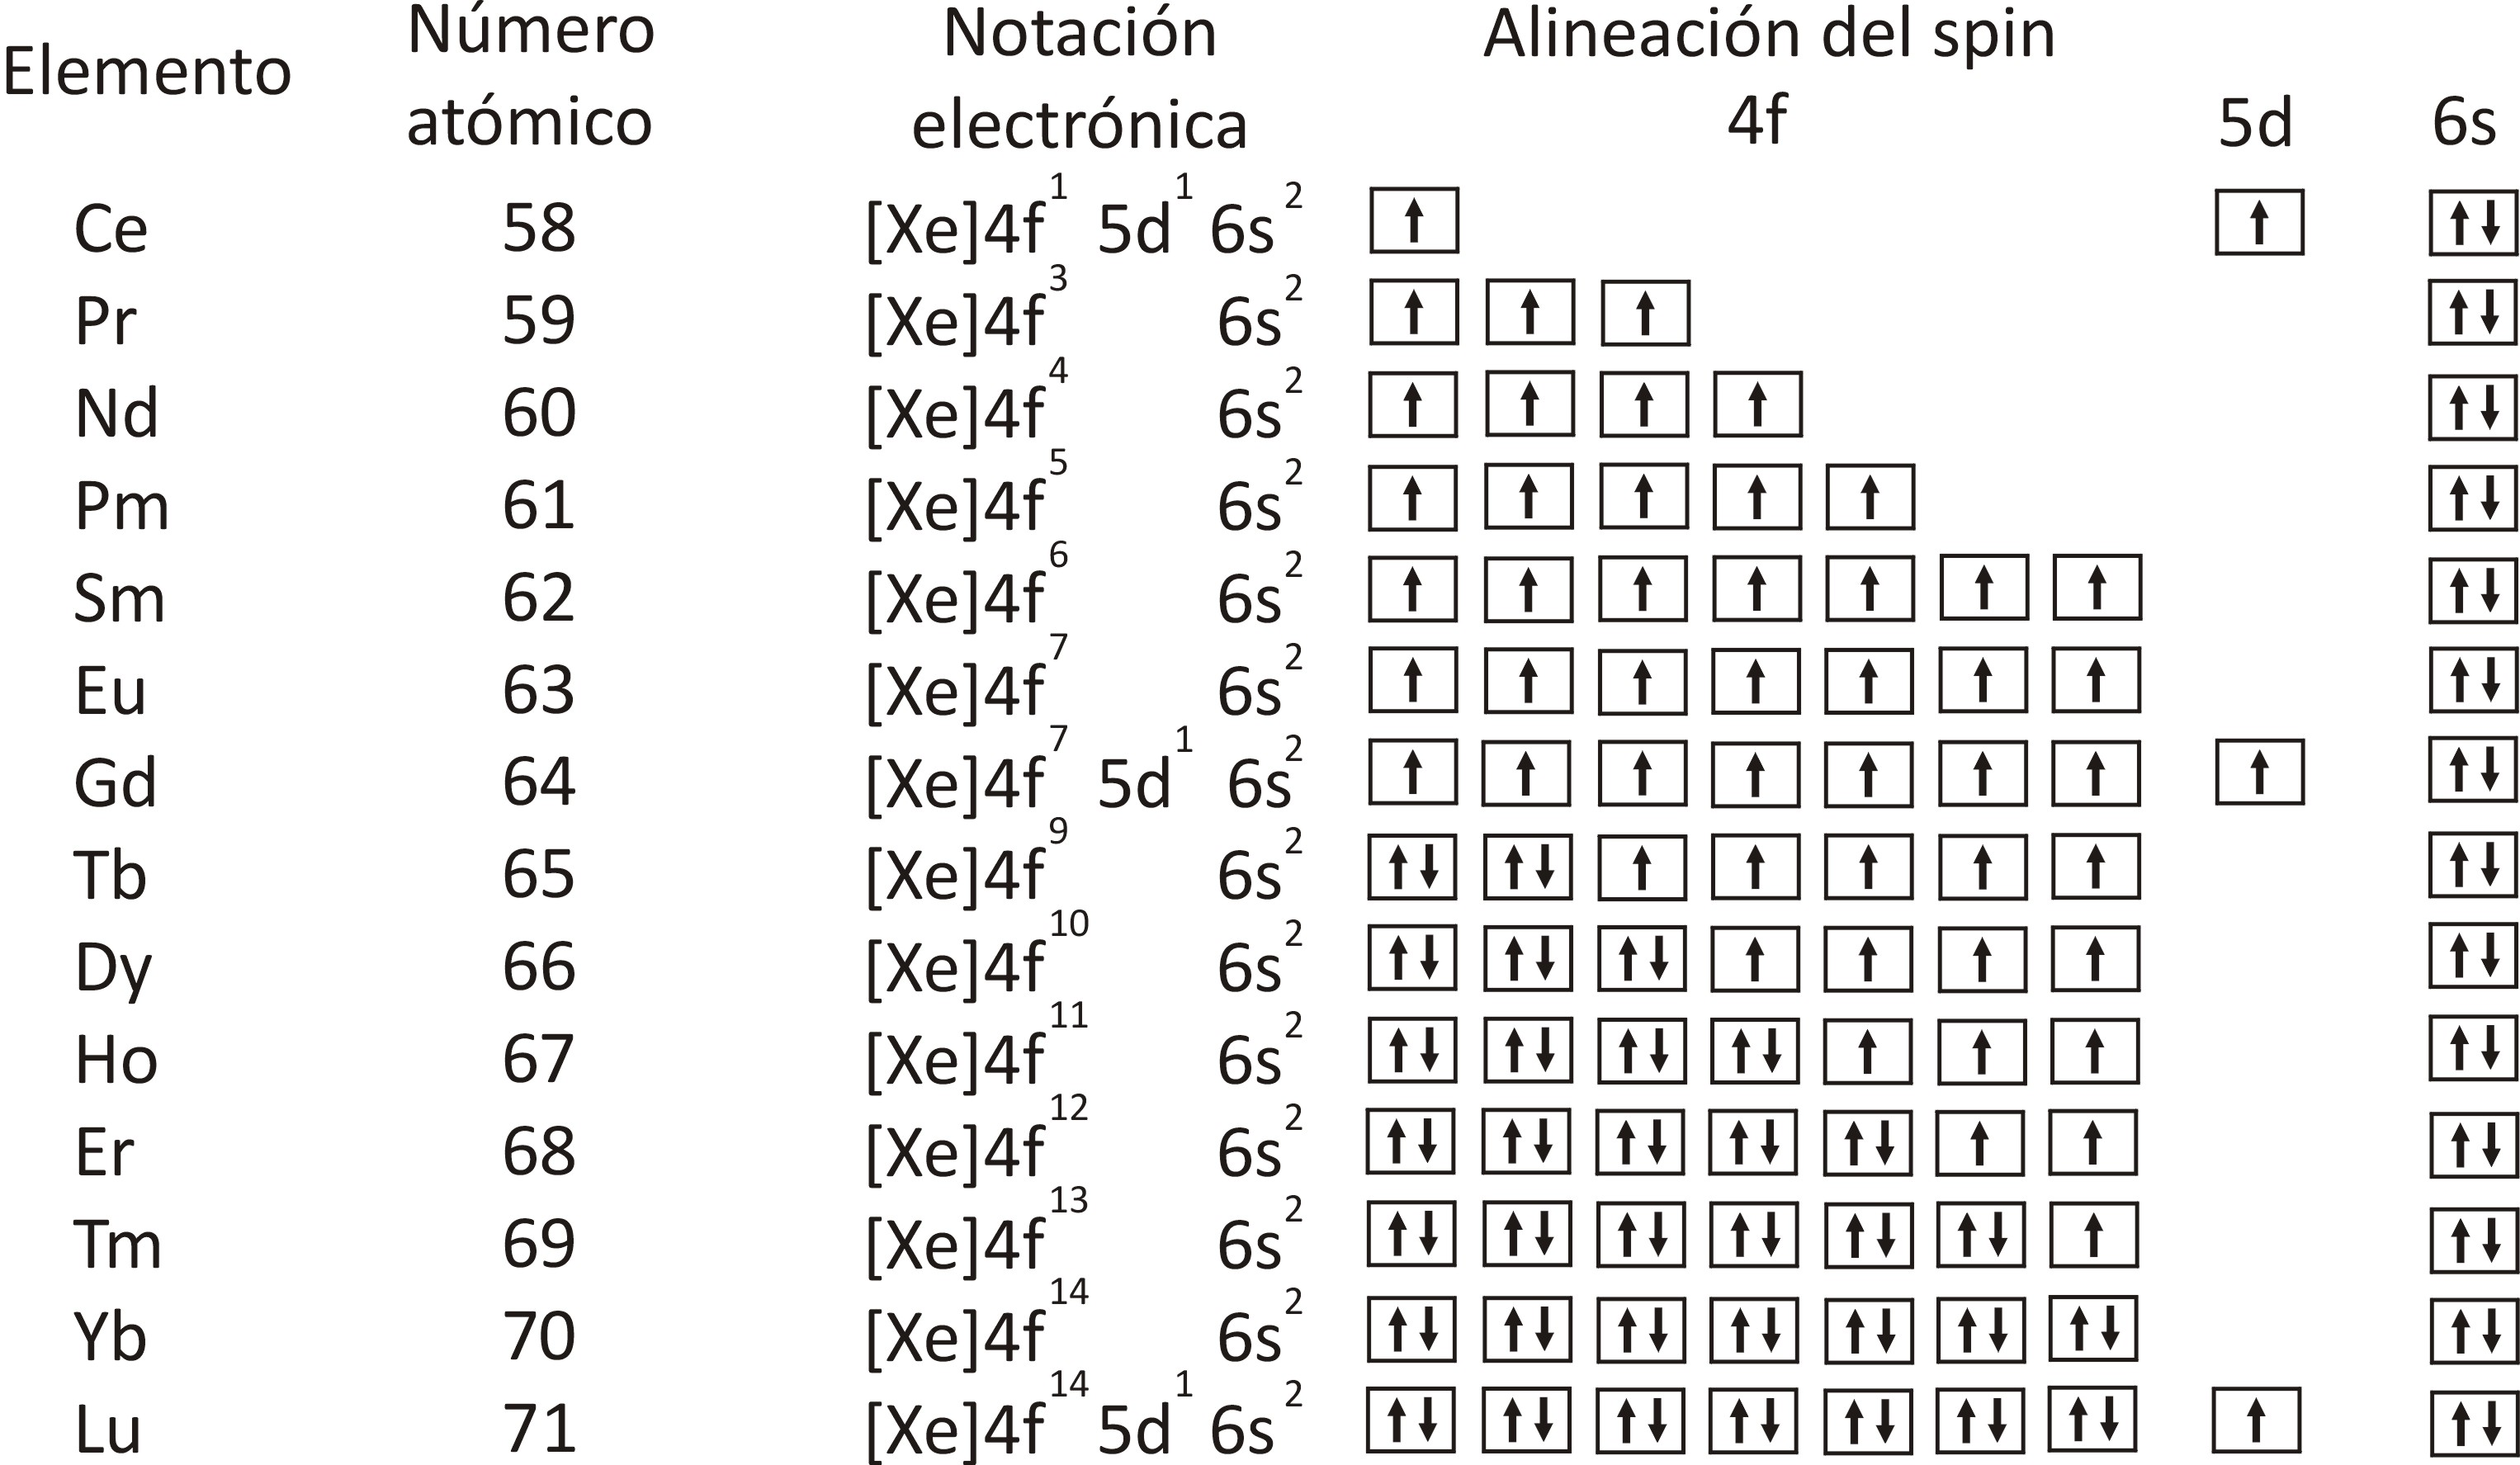
\includegraphics[width=1.0\textwidth]{./Figures/AlineacionDelEspin3grupo4f}
	\caption{Alineacion del espín grupo 4f}
	\label{fig:AlineacionDelEspin3grupo4f}
\end{figure}

Como se comento previamente los elementos de transición tienen el momento orbital bloqueado lo cual permite simplificar el cálculo del momento magnético atómico, pues solo debemos tener en cuenta el número de electrones no apareados.

\begin{equation}
	\mu_{j} = g_{j}\sqrt{j(j+1)}\,\mu_{B} \quad \text{luego} \quad \mu_{j}=2\sqrt{s(s+1)}\,\mu_{B}
\end{equation}

veamos el momento magnético de los iones de los elementos $3d$ en función del número $n$ de electrones
desapareados en unidades de $\mu_{B}$ magnetones de Bohr

\begin{equation}
	\mu_{j} = \sqrt{n(n+1)}\,\mu_{B} 
\end{equation}

\begin{figure}[H]
    \centering
    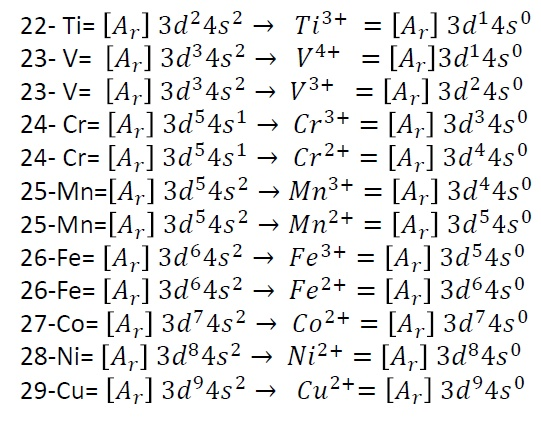
\includegraphics[width=0.8\textwidth]{./Figures/momMagElemTransicion3}
	\caption{Elementos de transición con momento orbital bloqueado}
	\label{fig:momMagElemTransicion3}
\end{figure}

\subsubsection{Momento magnético de los Elementos de transición interna}

\begin{figure}[H]
    \centering
    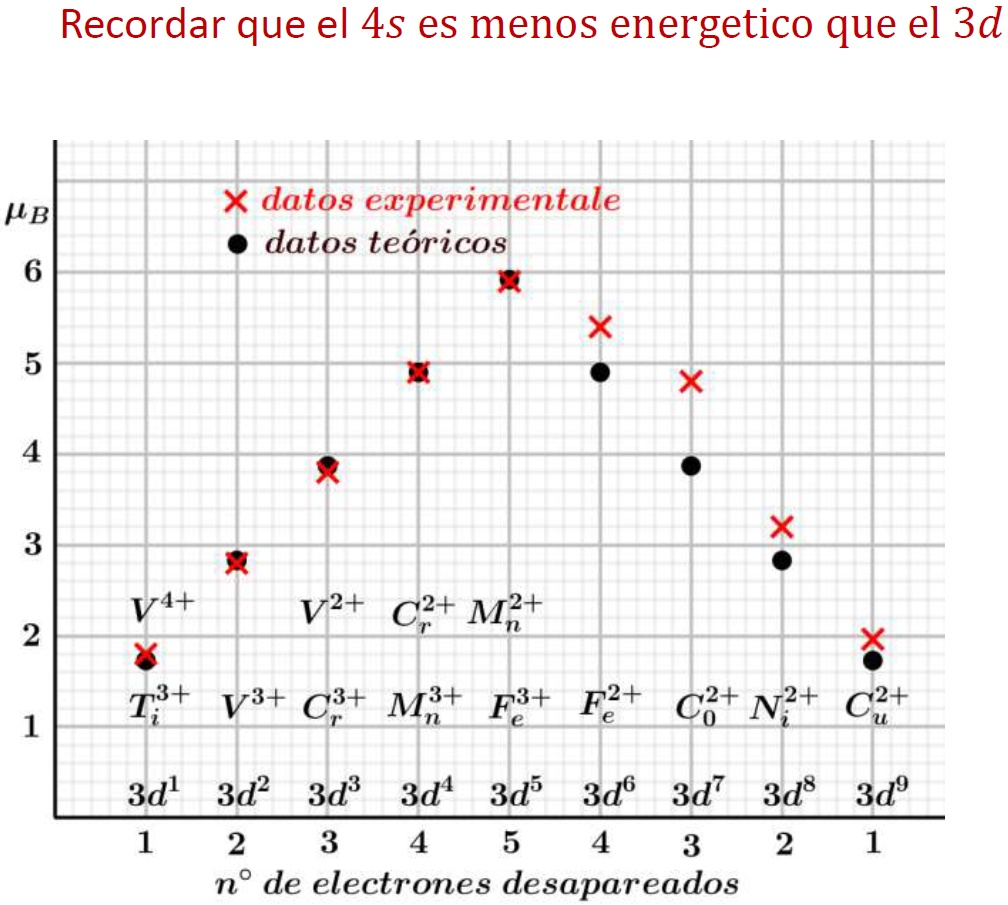
\includegraphics[width=1.0\textwidth]{./Figures/momMagElemTransicion2a}
	\caption{Momento magnético de los Elementos de transición interna}
	\label{fig:momMagElemTransicion2}
\end{figure}

\textbf{Tabla Periódica de los elementos que tienen electrones no apareados}

Los electrones no apareados les dan propiedades magnéticas al elemento en el que están y generalmente alteran sus propiedades ópticas

\begin{figure}[H]
    \centering
    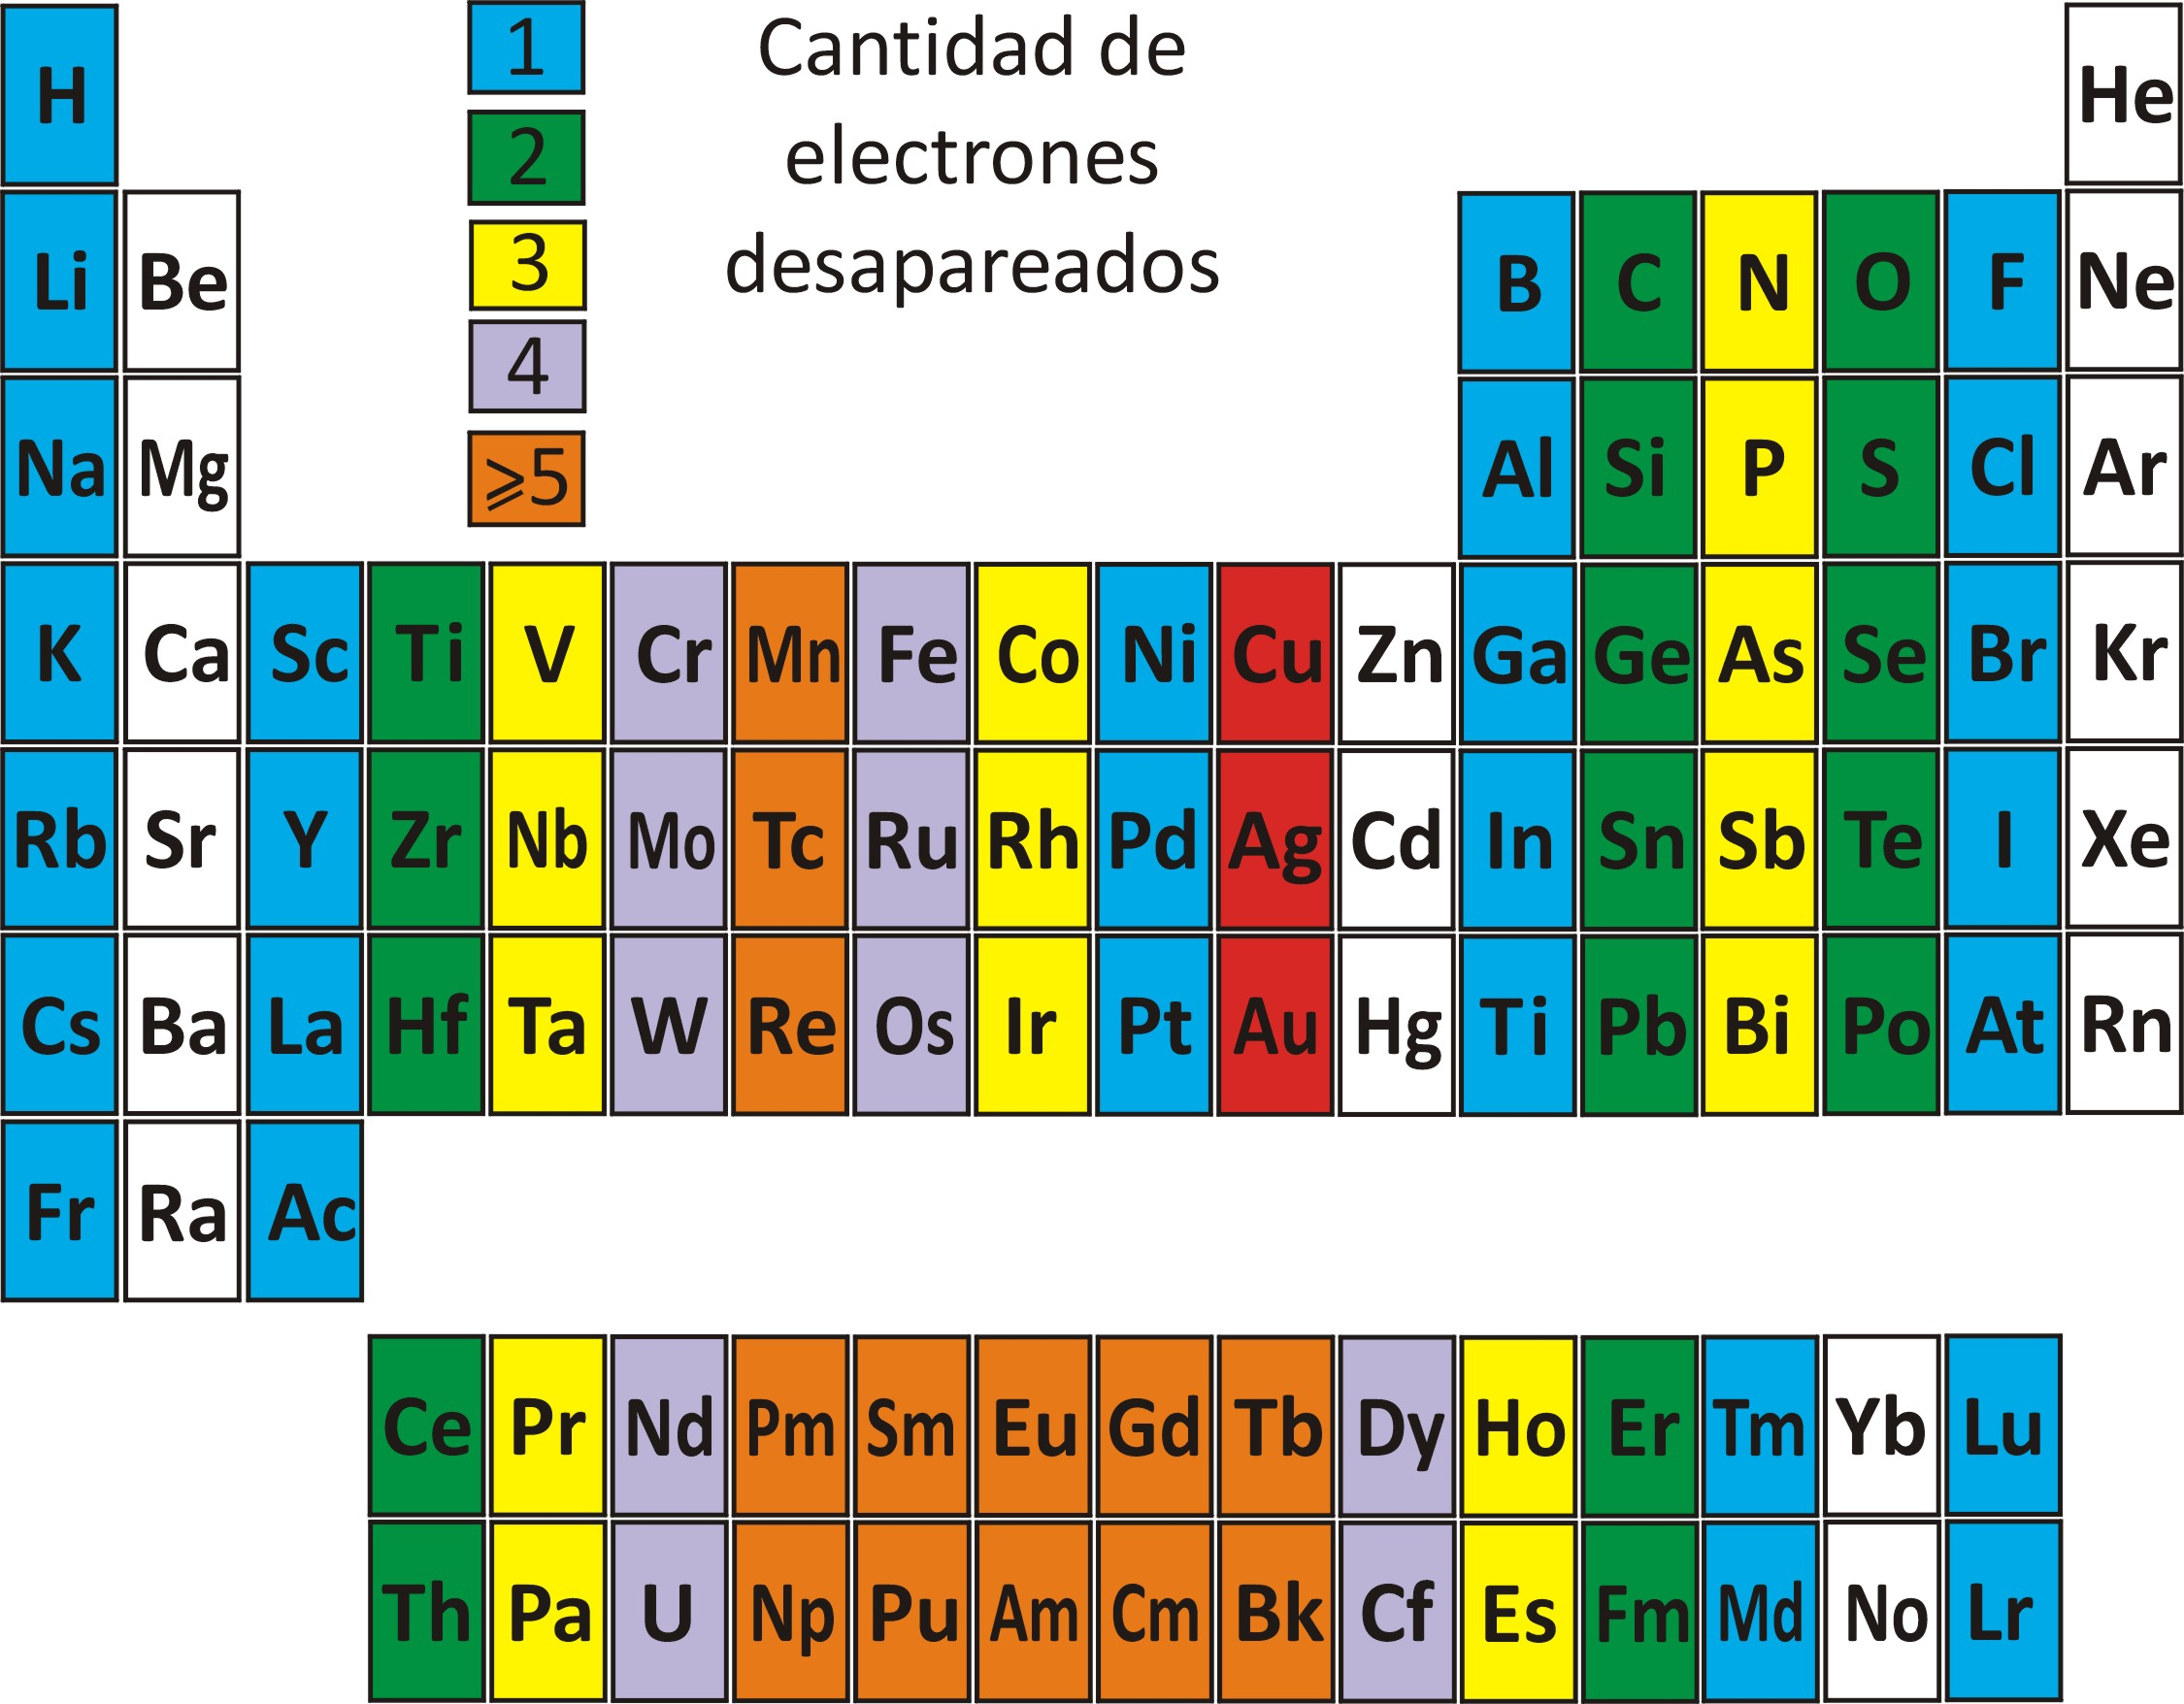
\includegraphics[width=1.0\textwidth]{./Figures/TablaPeriodica2}
	\caption{Elementos de electrones desapareados}
	\label{fig:TablaPeriodica2}
\end{figure}











